%%=============================================================================
%% Resultaten
%%=============================================================================

\chapter{Resultaten}%
\label{ch:resultaten}

\section{Resultaten}
\label{subsec:resultaatvisualisatie}

De evaluatie omvatte zes modellen die elk op 35 ETL taken werden getest, met drie samples per taak. Dit resulteerde in 630 individuele code evaluaties. De resultaten worden gevisualiseerd in de volgende figuren.

Uit de analyse blijkt een duidelijk verband tussen taakcomplexiteit en functionele correctheid. De taken werden ingedeeld in drie niveaus op basis van objectieve criteria: eenvoudige taken (1 bestand, 1 tot 2 standaardbewerkingen), gemiddelde taken (meerdere stappen, formaatherkenning of meerdere bestanden) en moeilijke taken (algoritmisch denken of geheugenefficiëntie). Voor eenvoudige taken varieerde de functionele correctheid van 44,4\% (mistral) tot 75,0\% (deepseek-coder-v2 en qwen2.5-coder). Voor gemiddelde taken daalde dit naar 20,0\% (mistral) tot 55,0\% (deepseek-coder-v2 en qwen2.5-coder). Alle zes modellen presteerden lager op gemiddelde dan op eenvoudige taken, wat bevestigt dat taken waarbij meerdere bewerkingen gecombineerd moeten worden, zoals inlezen, transformeren, valideren en wegschrijven, vaker tot fouten leiden. De moeilijke taken (chunked processing, memory filtering en fuzzy deduplication) vertoonden een wisselend beeld: deepseek-coder-v2 en qwen2.5-coder scoorden 66,7\%, gemma4 eveneens 66,7\%, terwijl phi4-mini slechts 11,1\% haalde.

De schaalbaarheidstest, waarbij de inputdata stapsgewijs werd vergroot tot het geheugengebruik de 2 GB grens overschreed, toonde eveneens duidelijke verschillen tussen de modellen. Qwen 2.5 Coder behaalde de hoogste gemiddelde schaalbaarheidsscore (80,6\%), gevolgd door Gemma 4 (79,9\%) en DeepSeek Coder V2 (77,2\%), terwijl Mistral de laagste score haalde (52,7\%). Opvallend is dat alle modellen voor bepaalde taken een schaalbaarheidsscore van 0\% noteerden, wat betekent dat de gegenereerde code wel correct werkte op kleine datasets maar faalde bij opschaling.

In Tabel~\ref{tab:pass_rates} wordt een volledig overzicht gegeven van de pass rates per evaluator per model.

\begin{table}[htbp]
\centering
\small
\setlength{\tabcolsep}{3.5pt}
\begin{tabular}{lcccccccc}
\toprule
\textbf{Model} & \textbf{Syntax} & \textbf{Style} & \textbf{Security} & \textbf{Exec.} & \textbf{Perf.} & \textbf{Radon} & \textbf{Funct.} & \textbf{Schaal.} \\
\midrule
DeepSeek Coder V2 & 100,0\% & 78,1\% & 100,0\% & 82,9\% & 81,9\% & 100,0\% & 57,1\% & 77,2\% \\
Gemma 4           & 100,0\% & 54,3\% & 100,0\% & 82,9\% & 82,9\% & 100,0\% & 58,1\% & 79,9\% \\
Llama 3           & 100,0\% & 81,9\% & 100,0\% & 62,9\% & 62,9\% & 100,0\% & 41,0\% & 65,5\% \\
Mistral           &  98,1\% & 76,2\% & 100,0\% & 51,4\% & 51,4\% &  98,1\% & 29,5\% & 52,7\% \\
Phi-4 Mini        &  95,2\% & 86,7\% & 100,0\% & 68,6\% & 68,6\% &  95,2\% & 36,2\% & 67,1\% \\
Qwen 2.5 Coder    & 100,0\% & 100,0\% & 100,0\% & 81,9\% & 81,9\% & 100,0\% & 57,1\% & 80,6\% \\
\bottomrule
\end{tabular}
\caption{Pass rate per evaluator per model over alle 105 samples (35 taken $\times$ 3 runs).}
\label{tab:pass_rates}
\end{table}

\textbf{Figuur \ref{fig:01_evaluator_comparison}} toont een gegroepeerd staafdiagram van het gemiddelde slagingspercentage per evaluator voor elk model. Qwen2.5-coder behaalde een perfecte score voor style (100\%) en excelleerde in syntax, security en Radon, maar bleef steken op 57,1\% voor functionele correctheid. Deepseek-coder-v2 toonde eveneens sterke syntactische en security resultaten met een functionele score van 57,1\%. Gemma4 had de hoogste functionele score (58,1\%) maar de laagste style compliance (54,3\%). Llama3 behaalde een degelijke overall score (81,7\%) maar liet lagere execution (62,9\%) en functionaliteit (41,0\%) zien. Phi4-mini en Mistral scoorden lager op functionaliteit, respectievelijk 36,2\% en 29,5\%, met Mistral ook opvallend zwak op execution (51,4\%).

\textbf{Figuur \ref{fig:functional_by_difficulty}} visualiseert de functionele correctheid per moeilijkheidsniveau. Alle zes modellen presteren lager op gemiddelde taken dan op eenvoudige taken. Voor eenvoudige taken varieert de functionele correctheid van 44,4\% (mistral) tot 75,0\% (deepseek-coder-v2 en qwen2.5-coder). Voor gemiddelde taken daalt deze naar 20,0\% (mistral) tot 55,0\% (deepseek-coder-v2 en qwen2.5-coder). De moeilijke taken (3 stuks) tonen een wisselend beeld, met uitschieters zoals phi4-mini (slechts 11,1\%).

\textbf{Figuur \ref{fig:overall_ranking}} toont de algemene rangschikking met drie scores per model. De rangschikking op kwaliteit (gemiddelde van de zes codekwaliteitsdimensies: syntaxis, style, security, executie, performantie en onderhoudbaarheid) is: deepseek-coder-v2 (90,3\%), qwen2.5-coder (90,2\%), gemma4 (86,5\%), phi4-mini (85,4\%), llama3 (81,7\%) en mistral (79,6\%). Gemma 4 behaalt de hoogste functionele score (58,1\%), Qwen 2.5 Coder de beste schaalbaarheid (80,6\%).

\textbf{Figuur \ref{fig:scalability}} toont de schaalbaarheidsscore per model met het minimale en maximale bereik. Alle modellen hebben voor sommige taken een score van 0\%, wat betekent dat de code wel werkte op kleine datasets maar faalde bij opschaling.

\textbf{Figuur \ref{fig:maintainability}} toont de onderhoudbaarheidsindex (Radon) per model. Alle modellen scoorden uitstekend, met waarden boven de 95\%.

\textbf{Figuur \ref{fig:execution_times}} toont de verdeling van de uitvoeringstijden per model. Dit geeft inzicht in de runtime-efficiëntie van de gegenereerde code.

\textbf{Figuur \ref{fig:lines_of_code}} geeft een weergave van de code omvang per model.

\textbf{Figuur \ref{fig:08_sample_consistency}} toont de consistentie over de drie samples per evaluator. Een lagere variantie wijst op een betrouwbaardere codegeneratie.

\textbf{Figuur \ref{fig:09_generation_speed}} toont de generatiesnelheid in tokens per seconde voor elk model.

\begin{figure}[htbp]
    \centering
    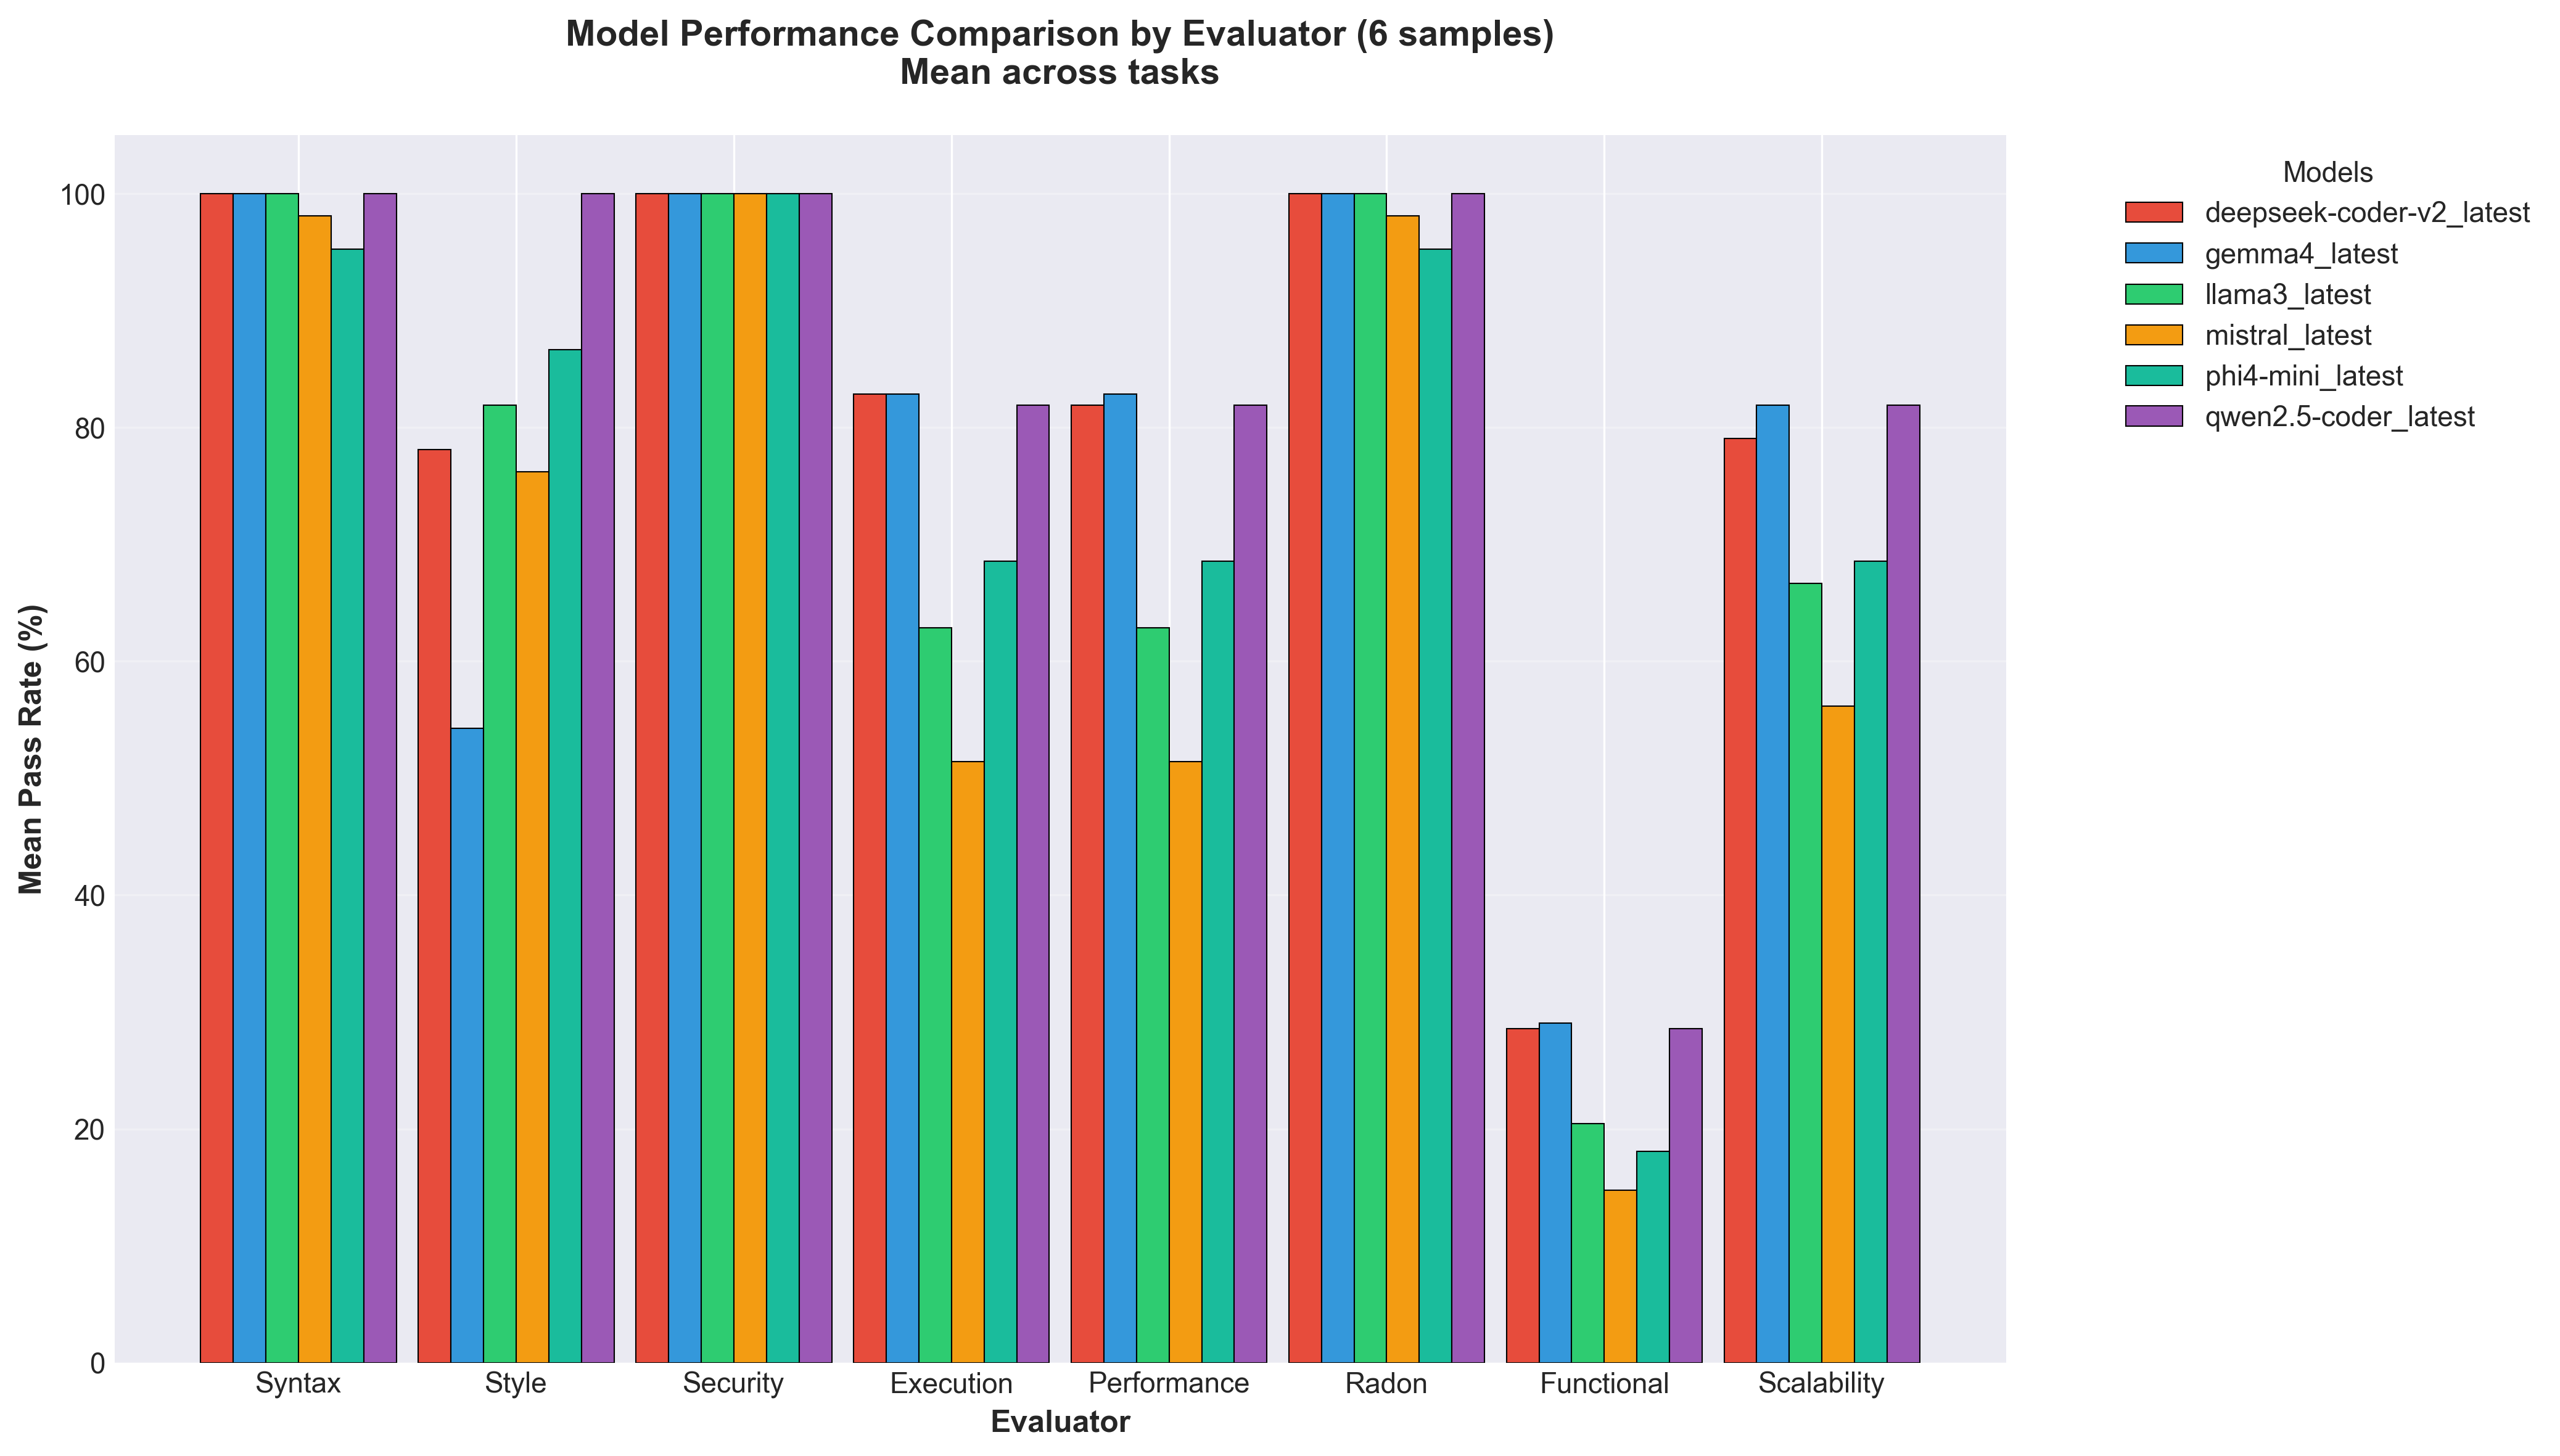
\includegraphics[width=0.9\linewidth]{images/01_evaluator_comparison.png}
    \caption{Vergelijking van de gemiddelde slagingspercentages per evaluator voor alle zes modellen. De figuur toont aan dat alle modellen hoog scoren op syntax, beveiliging en onderhoudbaarheid, maar dat de functionele correctheid (29,5\% tot 58,1\%) systematisch het grootste knelpunt vormt.}
    \label{fig:01_evaluator_comparison}
\end{figure}

\begin{figure}[htbp]
    \centering
    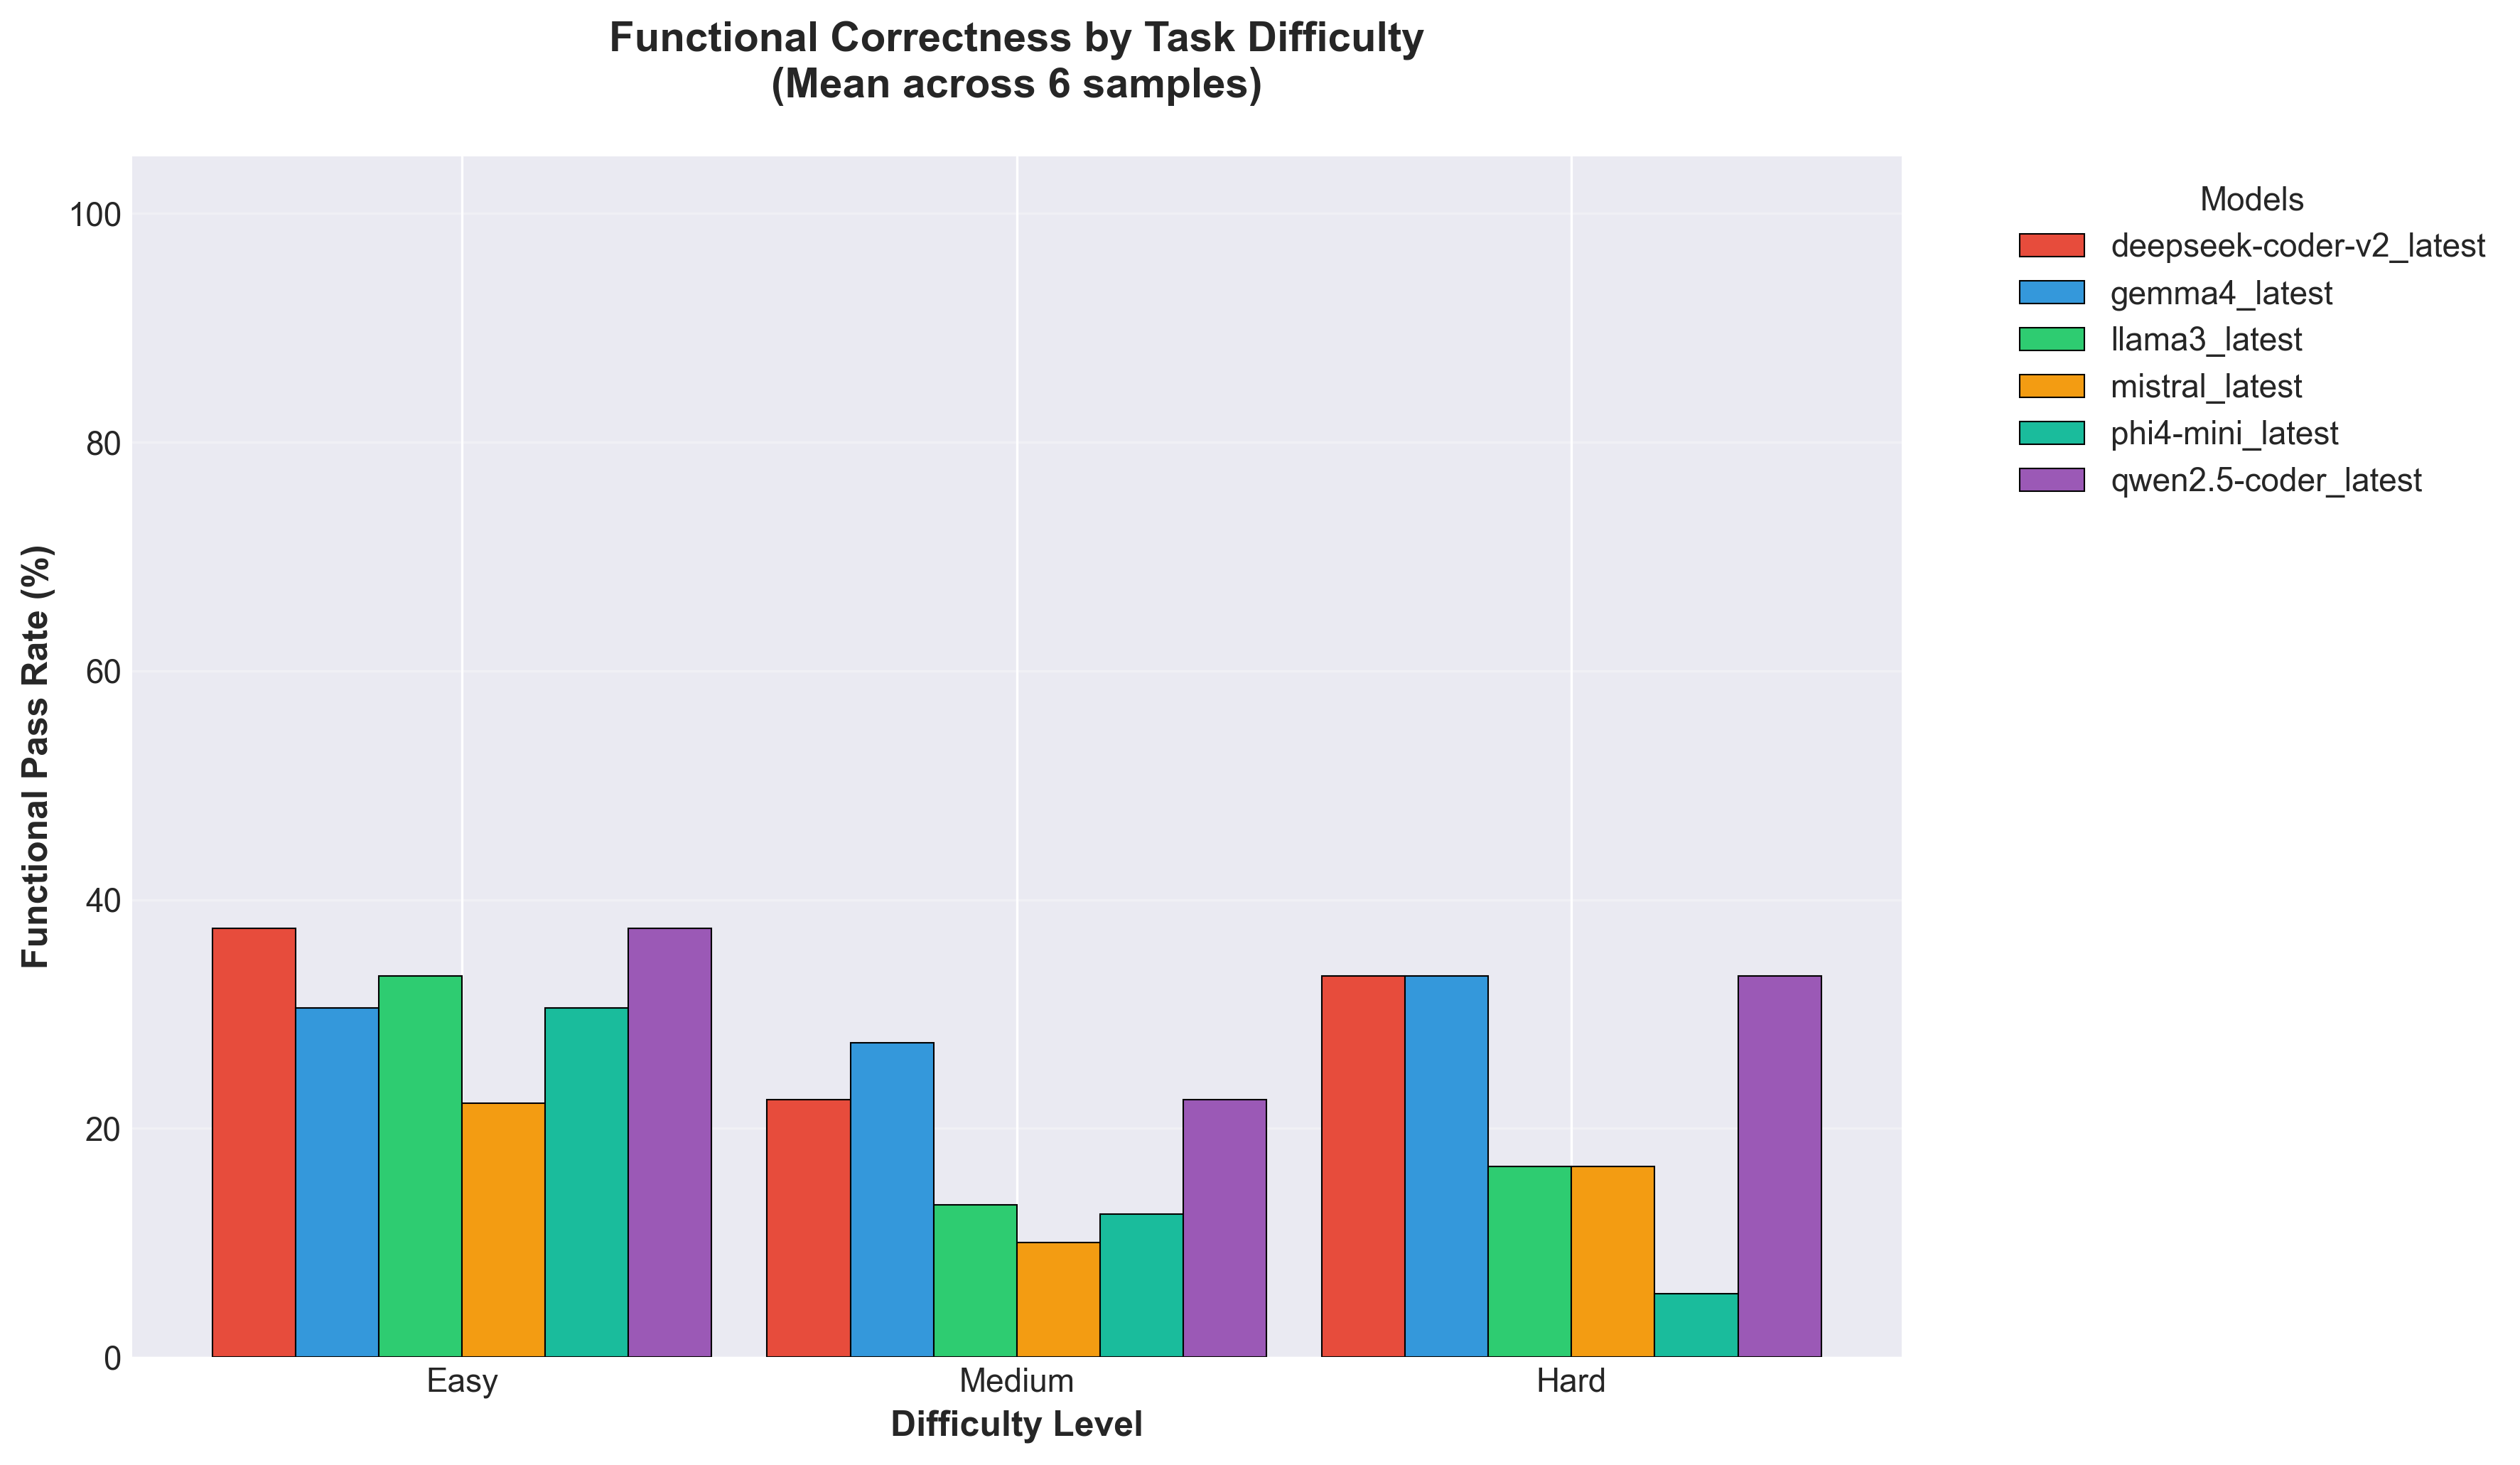
\includegraphics[width=0.9\linewidth]{images/02_functional_by_difficulty.png}
    \caption{Functionele correctheid per moeilijkheidsniveau (eenvoudig, gemiddeld, moeilijk). Alle zes modellen presteren lager op gemiddelde dan op eenvoudige taken.}
    \label{fig:functional_by_difficulty}
\end{figure}

\begin{figure}[htbp]
    \centering
    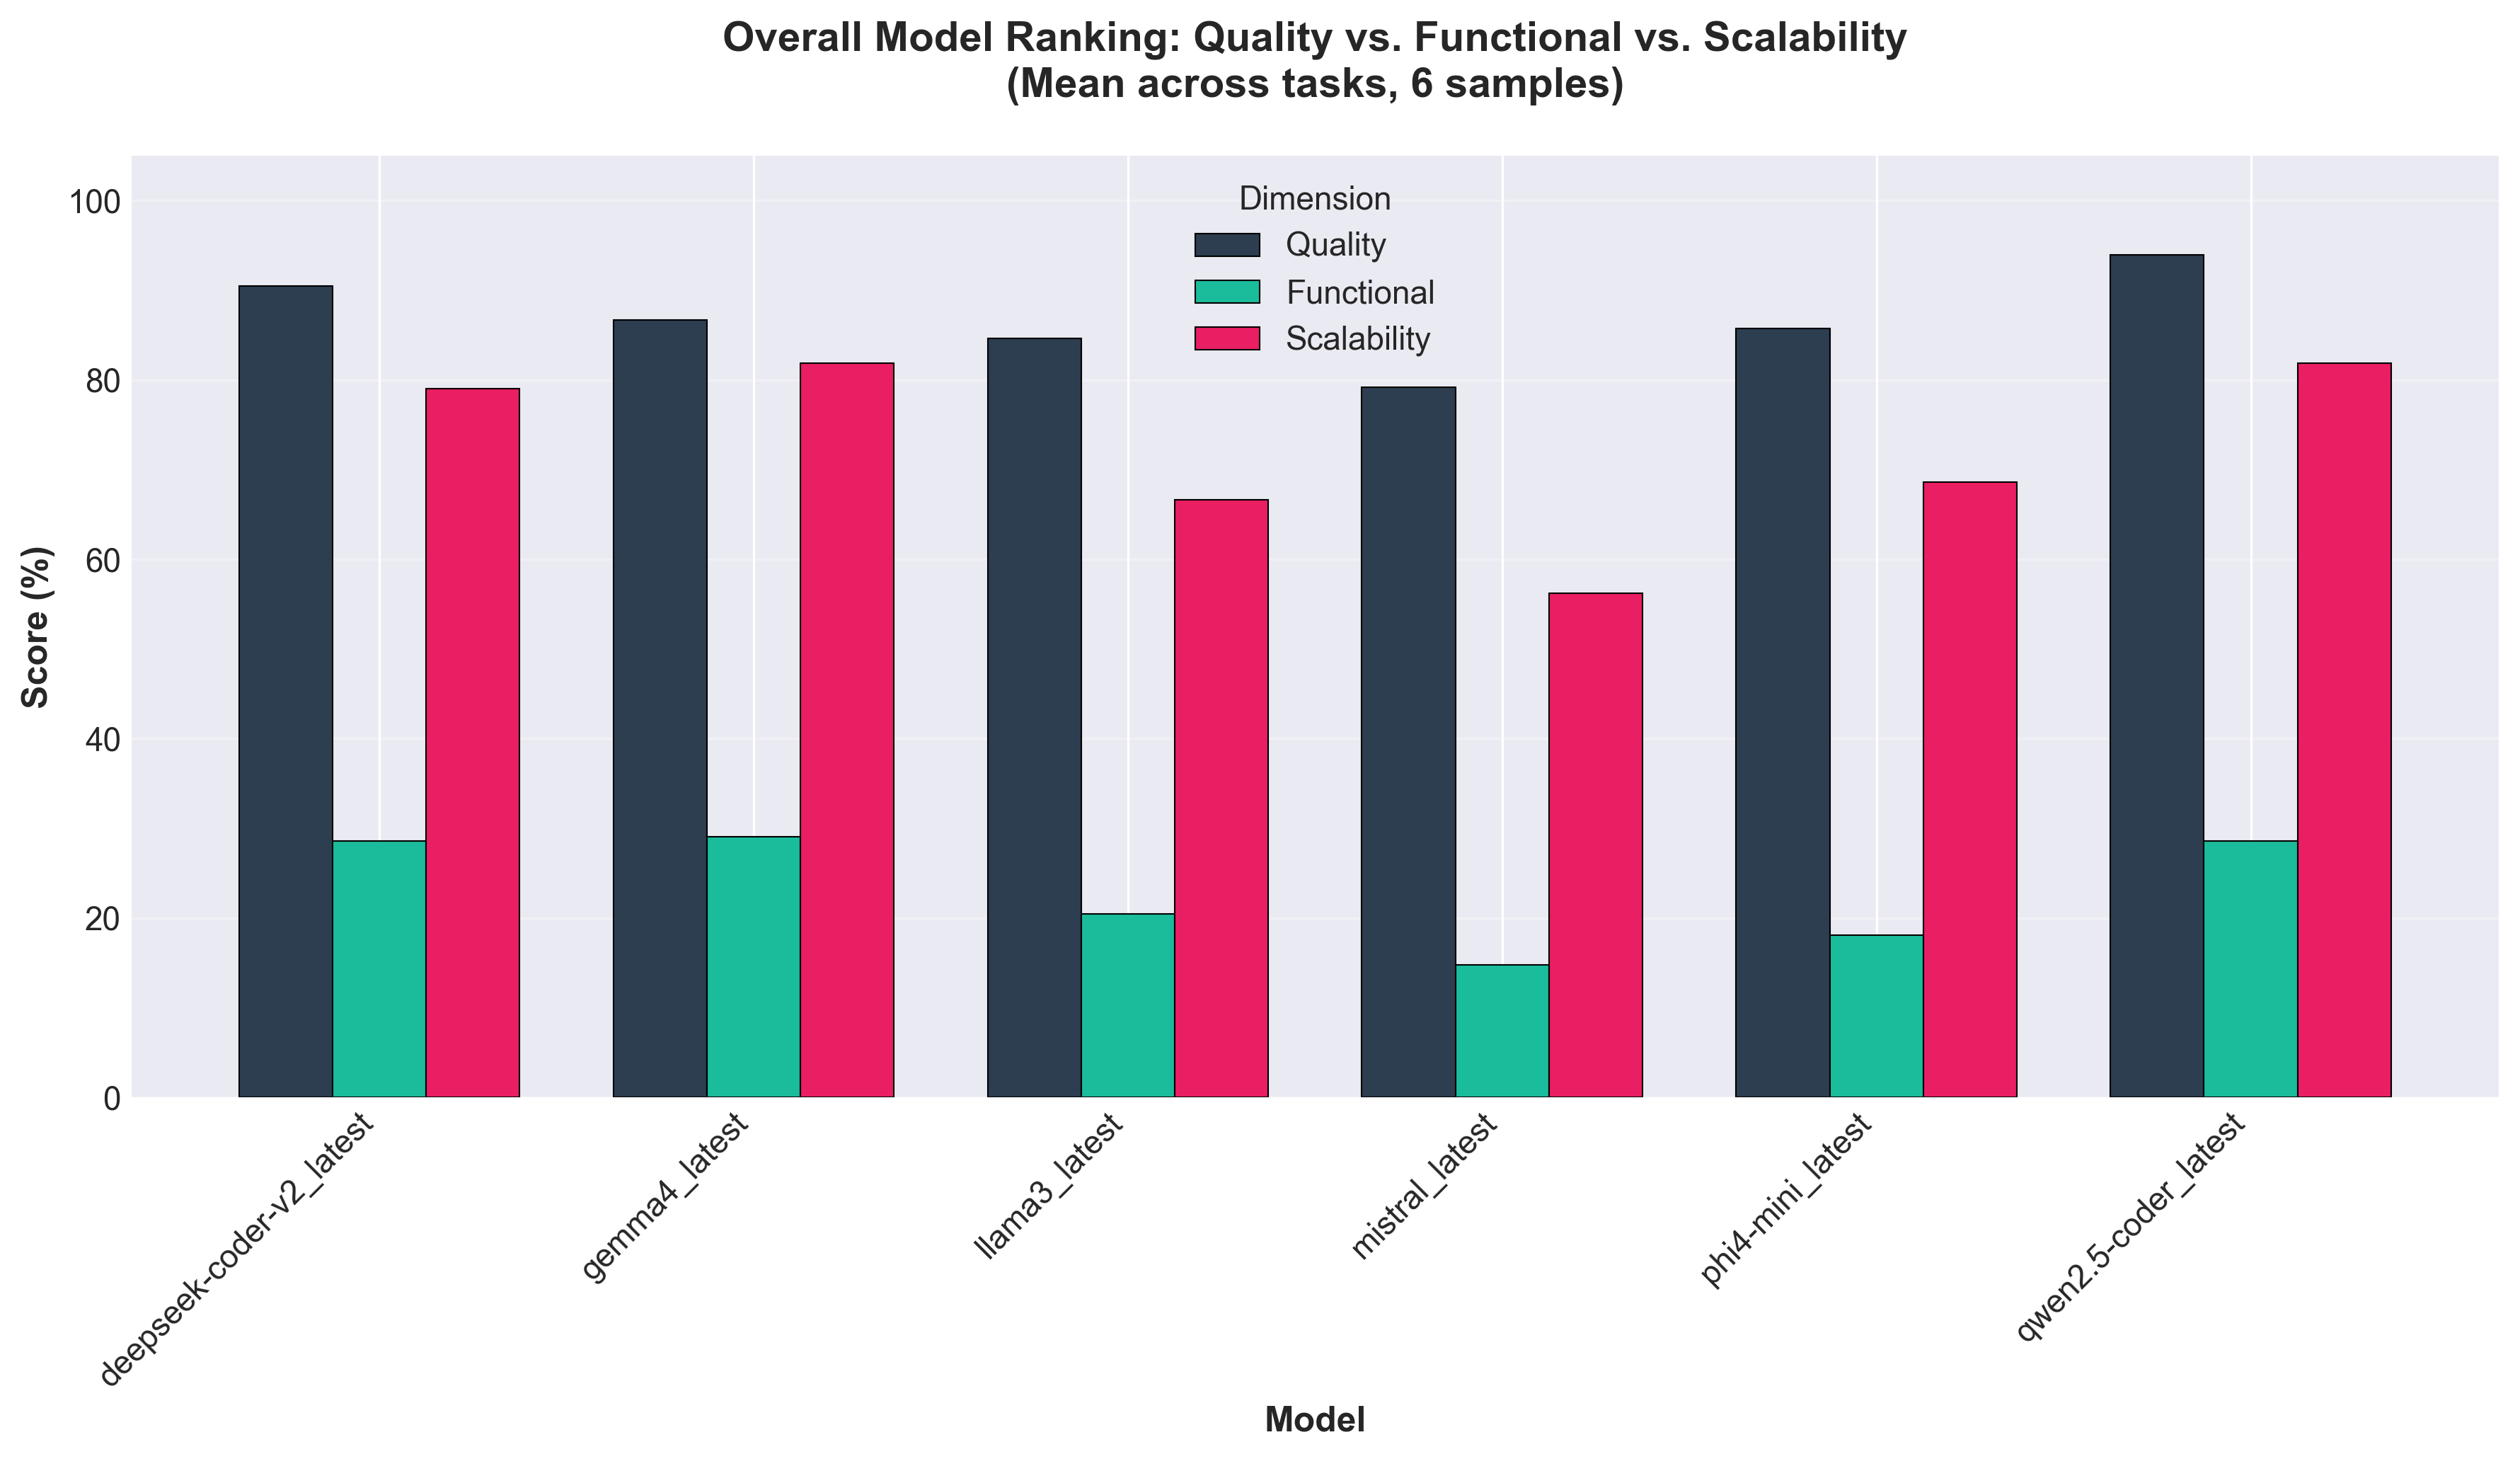
\includegraphics[width=0.9\linewidth]{images/03_overall_ranking.png}
    \caption{Eindranking met kwaliteit (6 evaluatoren), functionele correctheid en schaalbaarheid per model. DeepSeek Coder V2 voert aan op kwaliteit (90,3\%), Gemma 4 op functionele correctheid (58,1\%) en Qwen 2.5 Coder op schaalbaarheid (80,6\%).}
    \label{fig:overall_ranking}
\end{figure}

\begin{figure}[htbp]
    \centering
    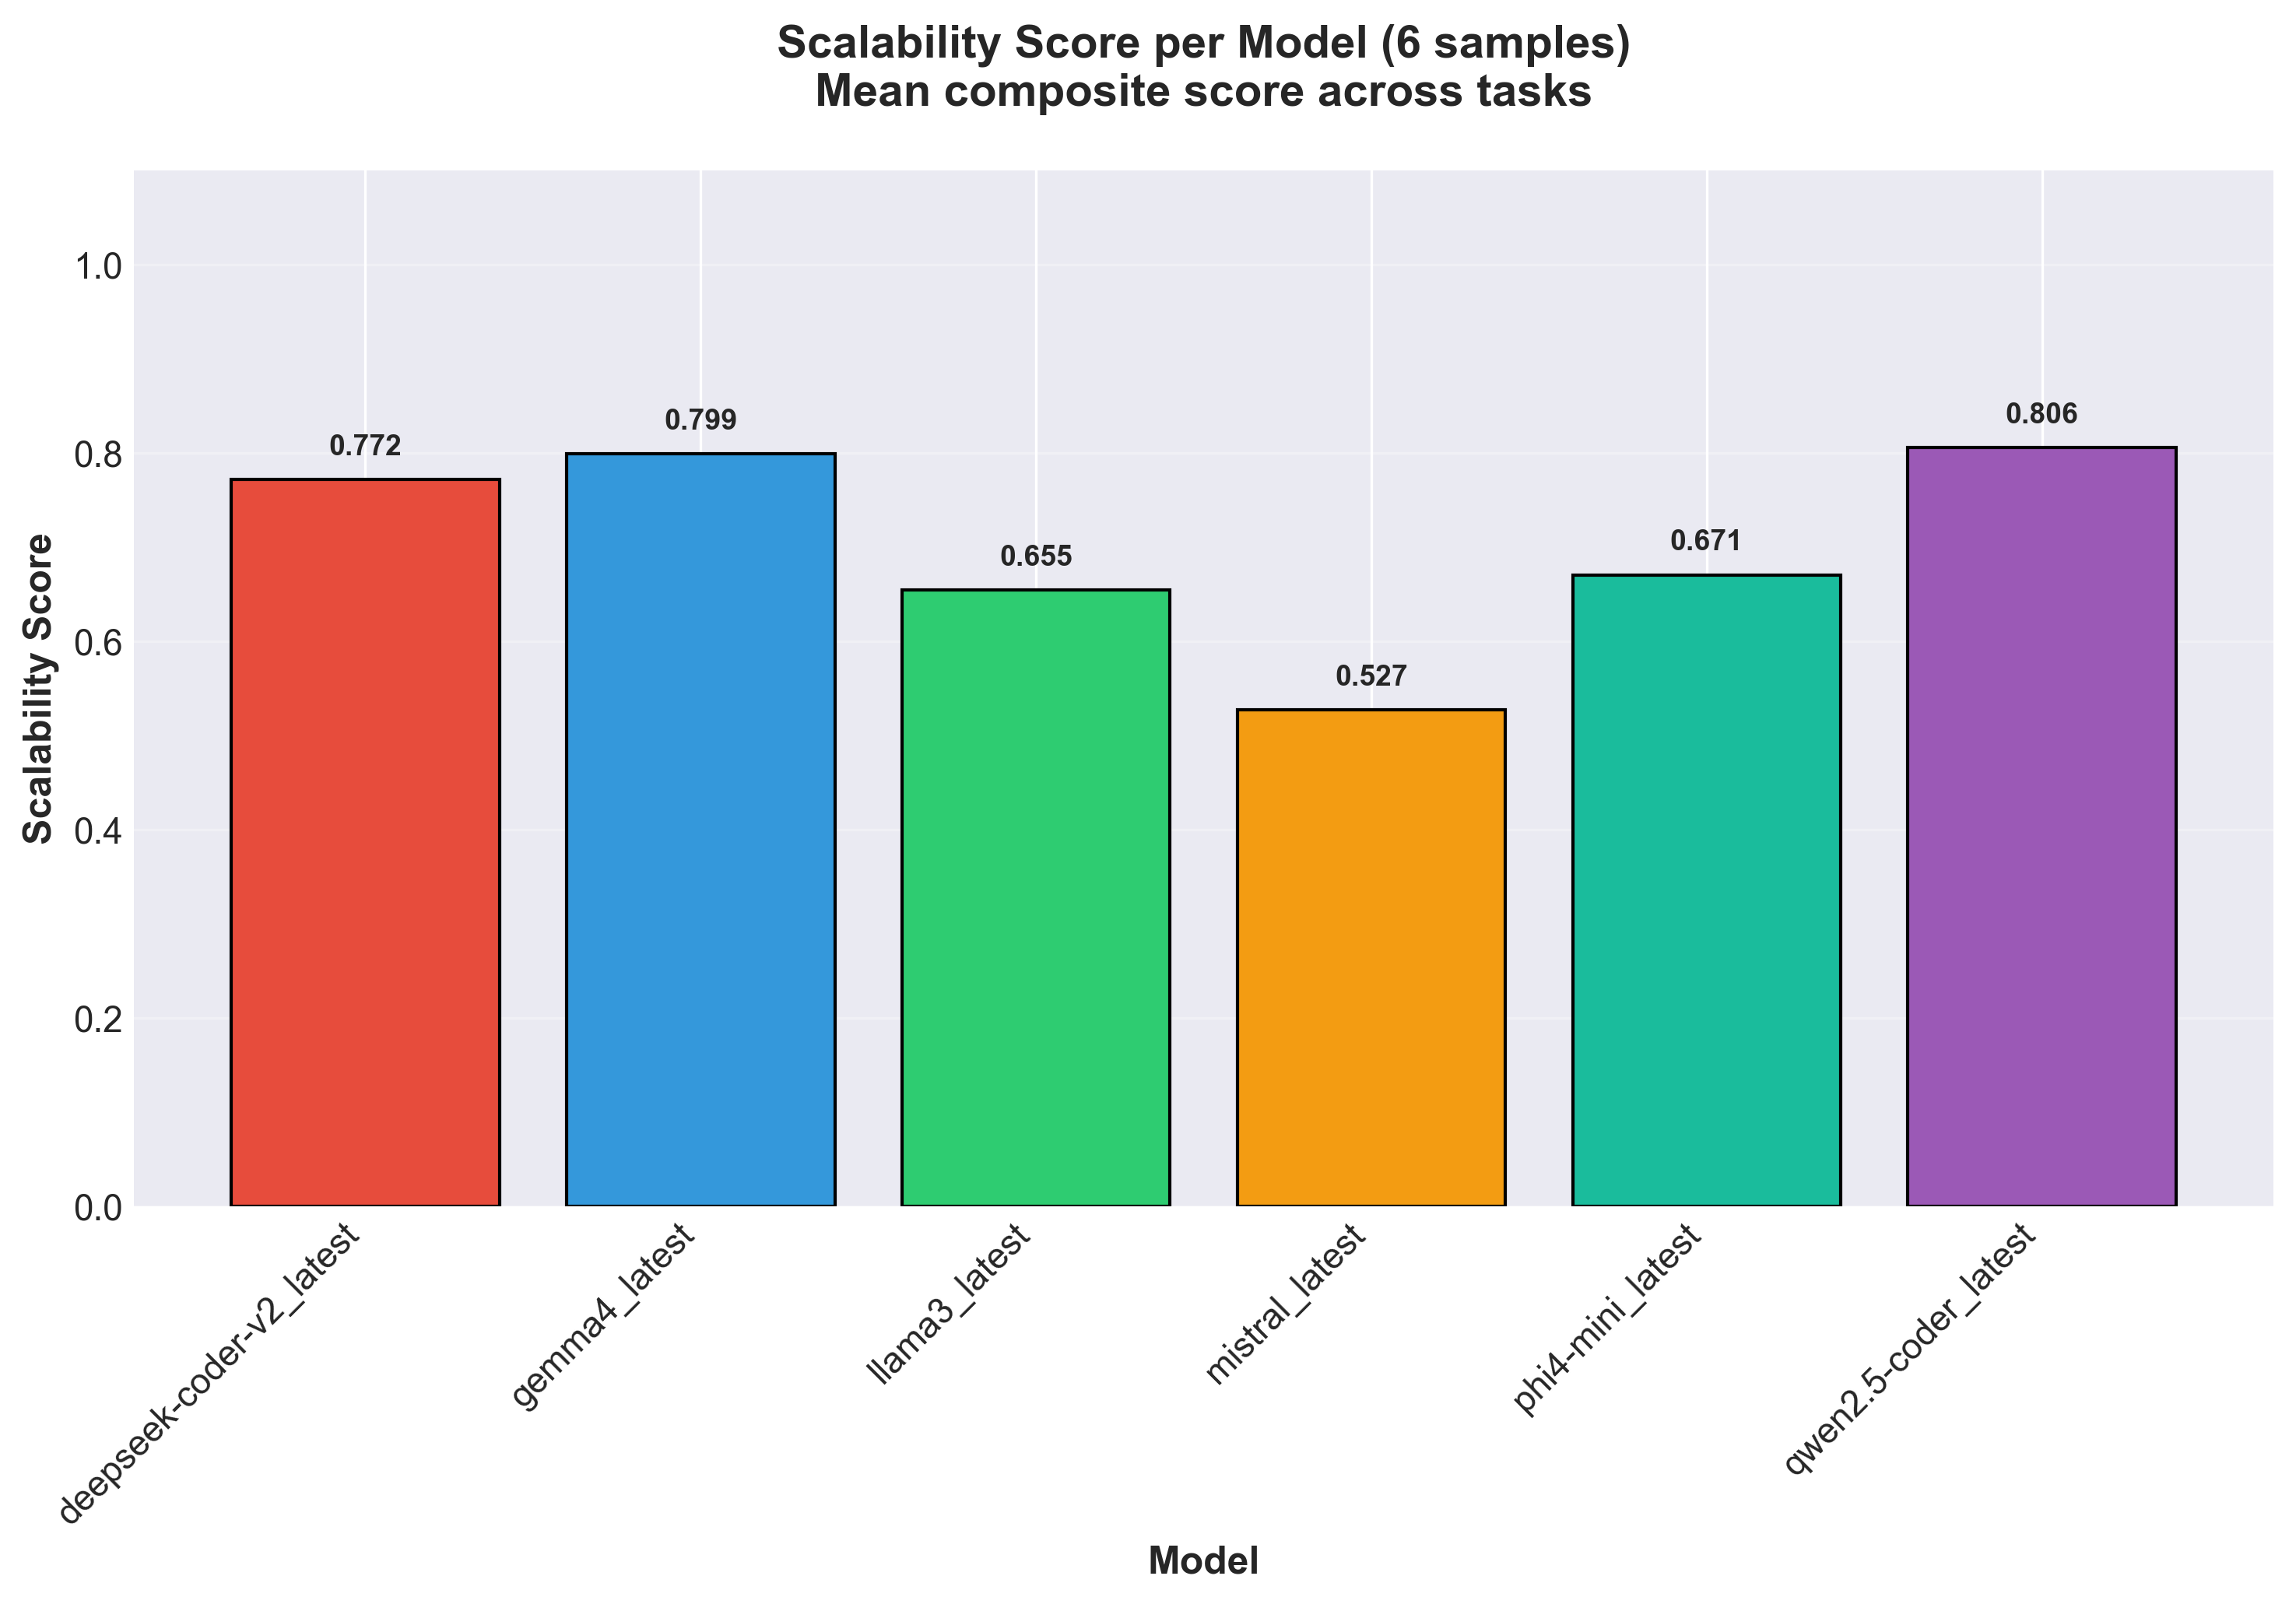
\includegraphics[width=0.9\linewidth]{images/04_scalability.png}
    \caption{Schaalbaarheidsscore per model met minimale en maximale waarden. De figuur toont dat Qwen 2.5 Coder het beste presteert op schaalbaarheid (80,6\%) en Mistral het zwakst (52,7\%).}
    \label{fig:scalability}
\end{figure}

\begin{figure}[htbp]
    \centering
    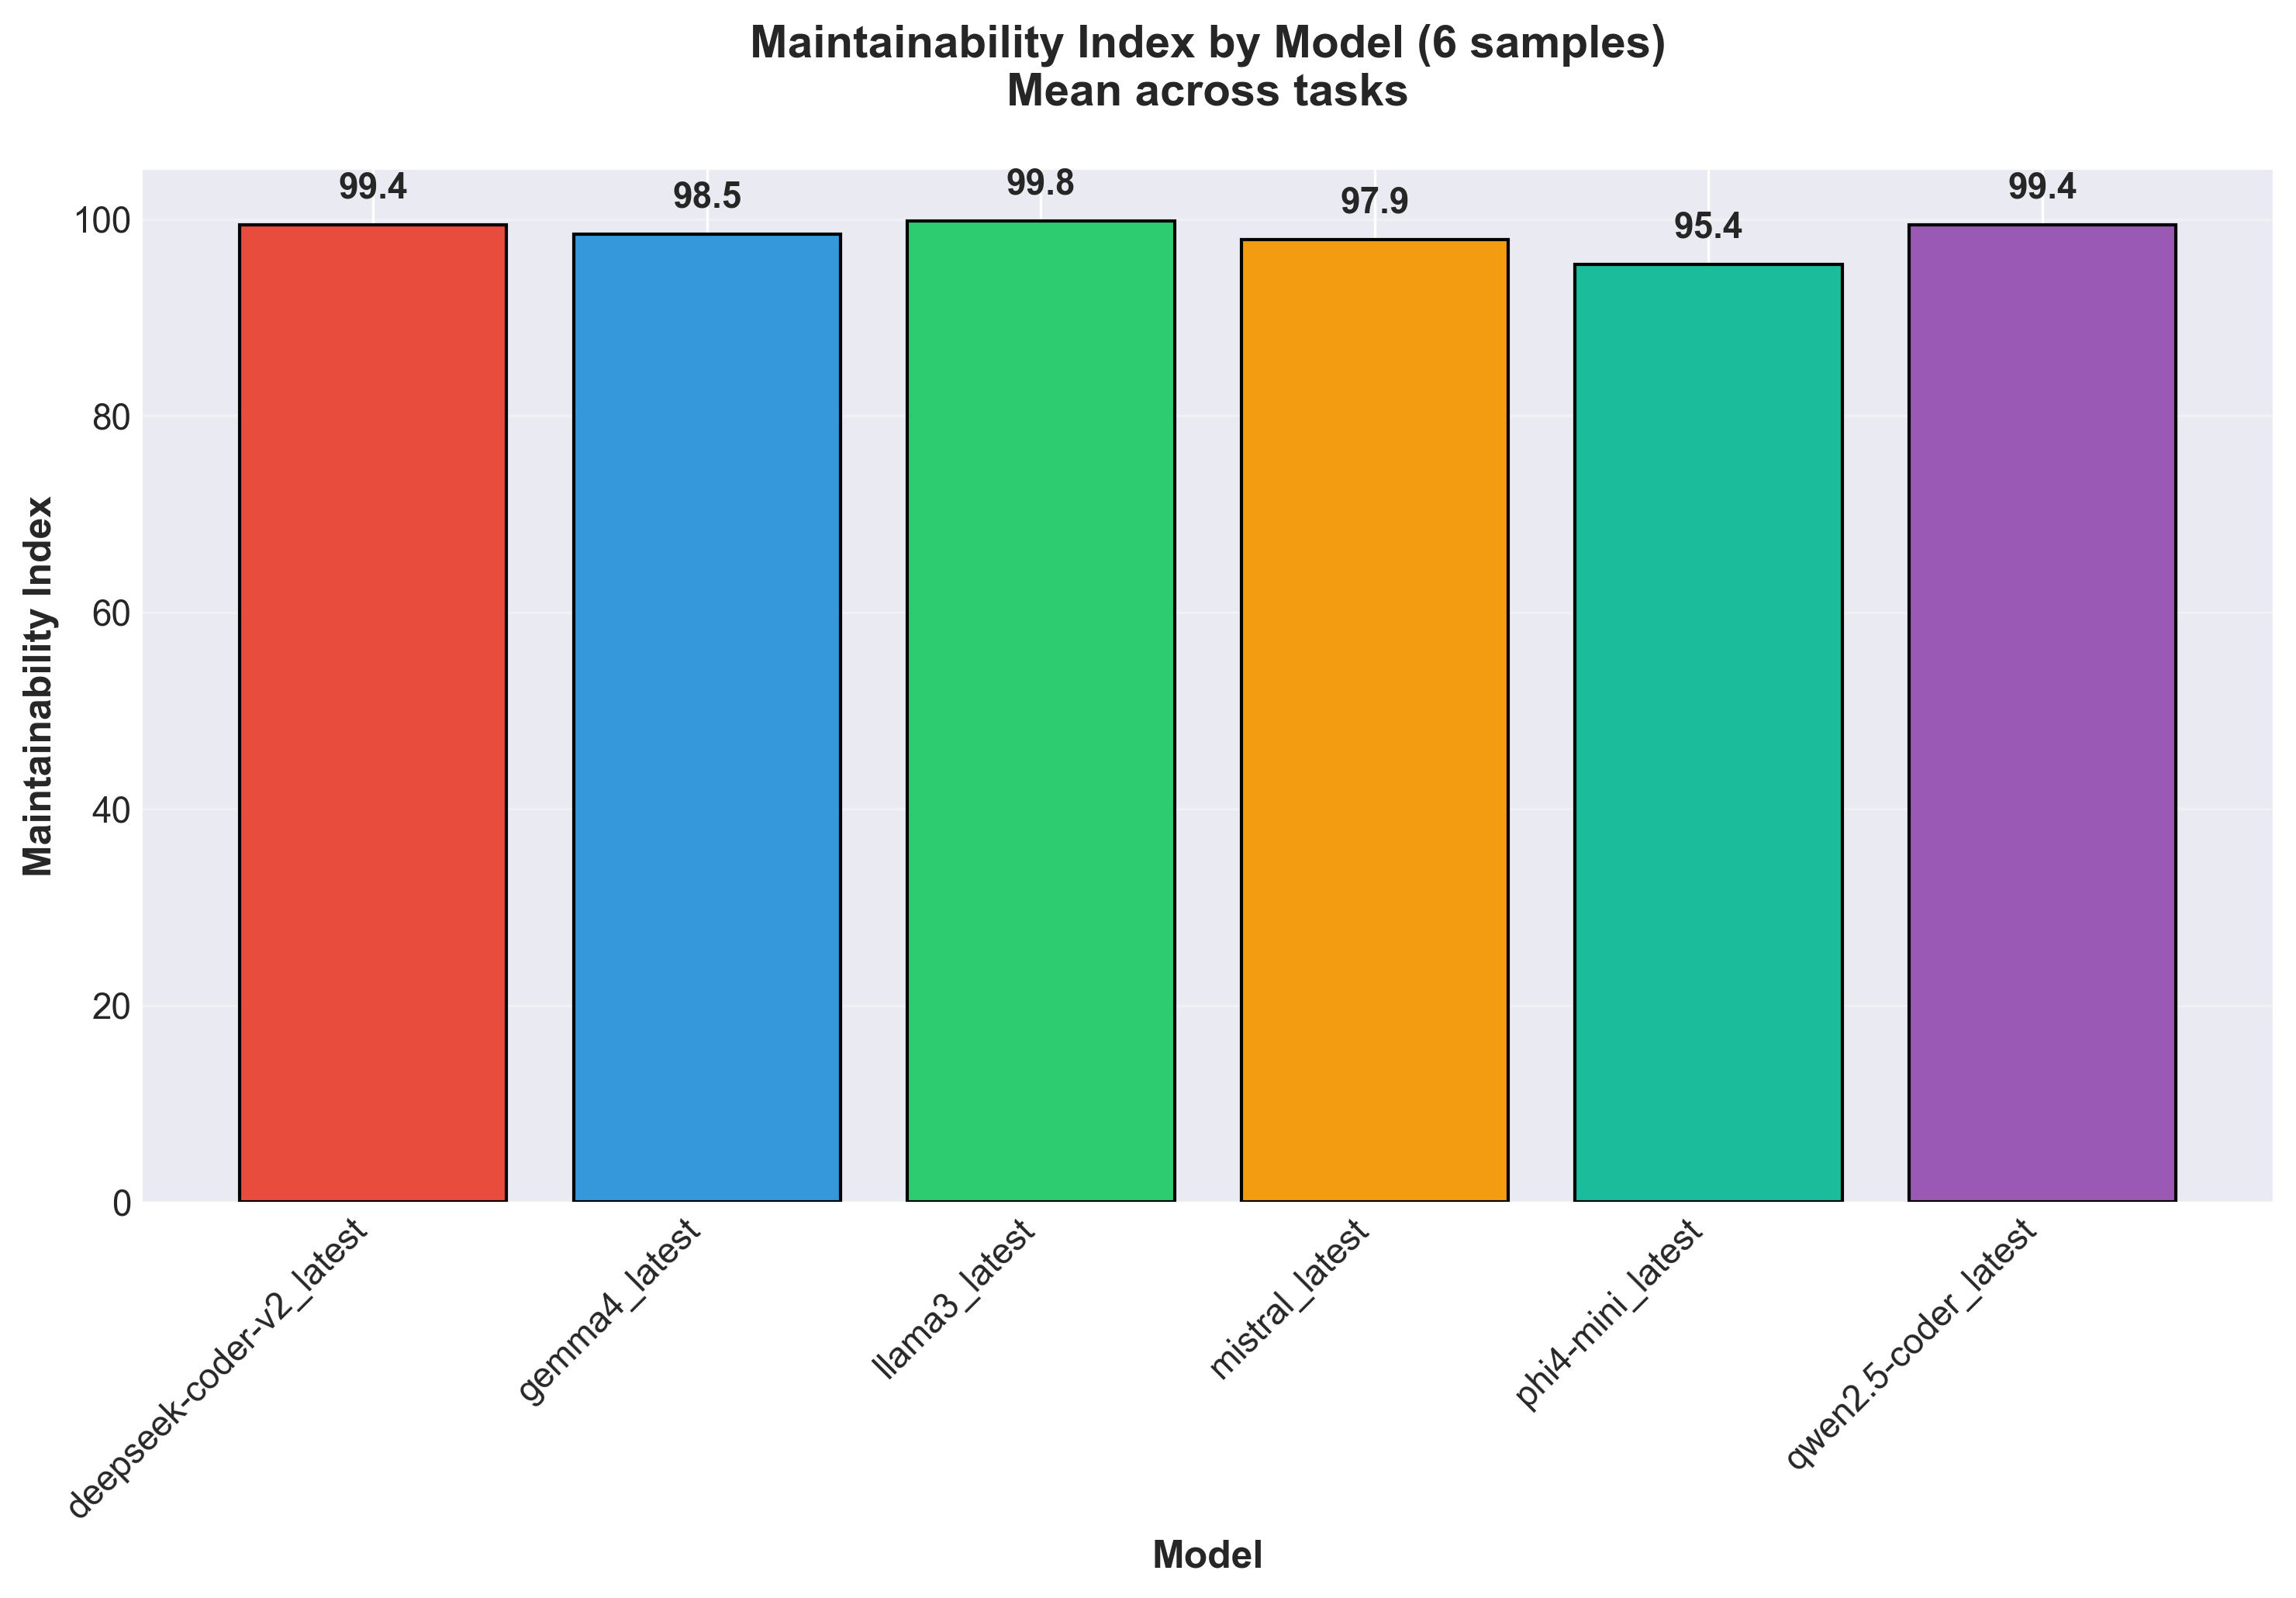
\includegraphics[width=0.9\linewidth]{images/05_maintainability.png}
    \caption{Onderhoudbaarheidsindex (Radon) per model, weergegeven als gemiddelde met standaarddeviatie. Alle modellen behalen waarden boven 95\%.}
    \label{fig:maintainability}
\end{figure}

\begin{figure}[htbp]
    \centering
    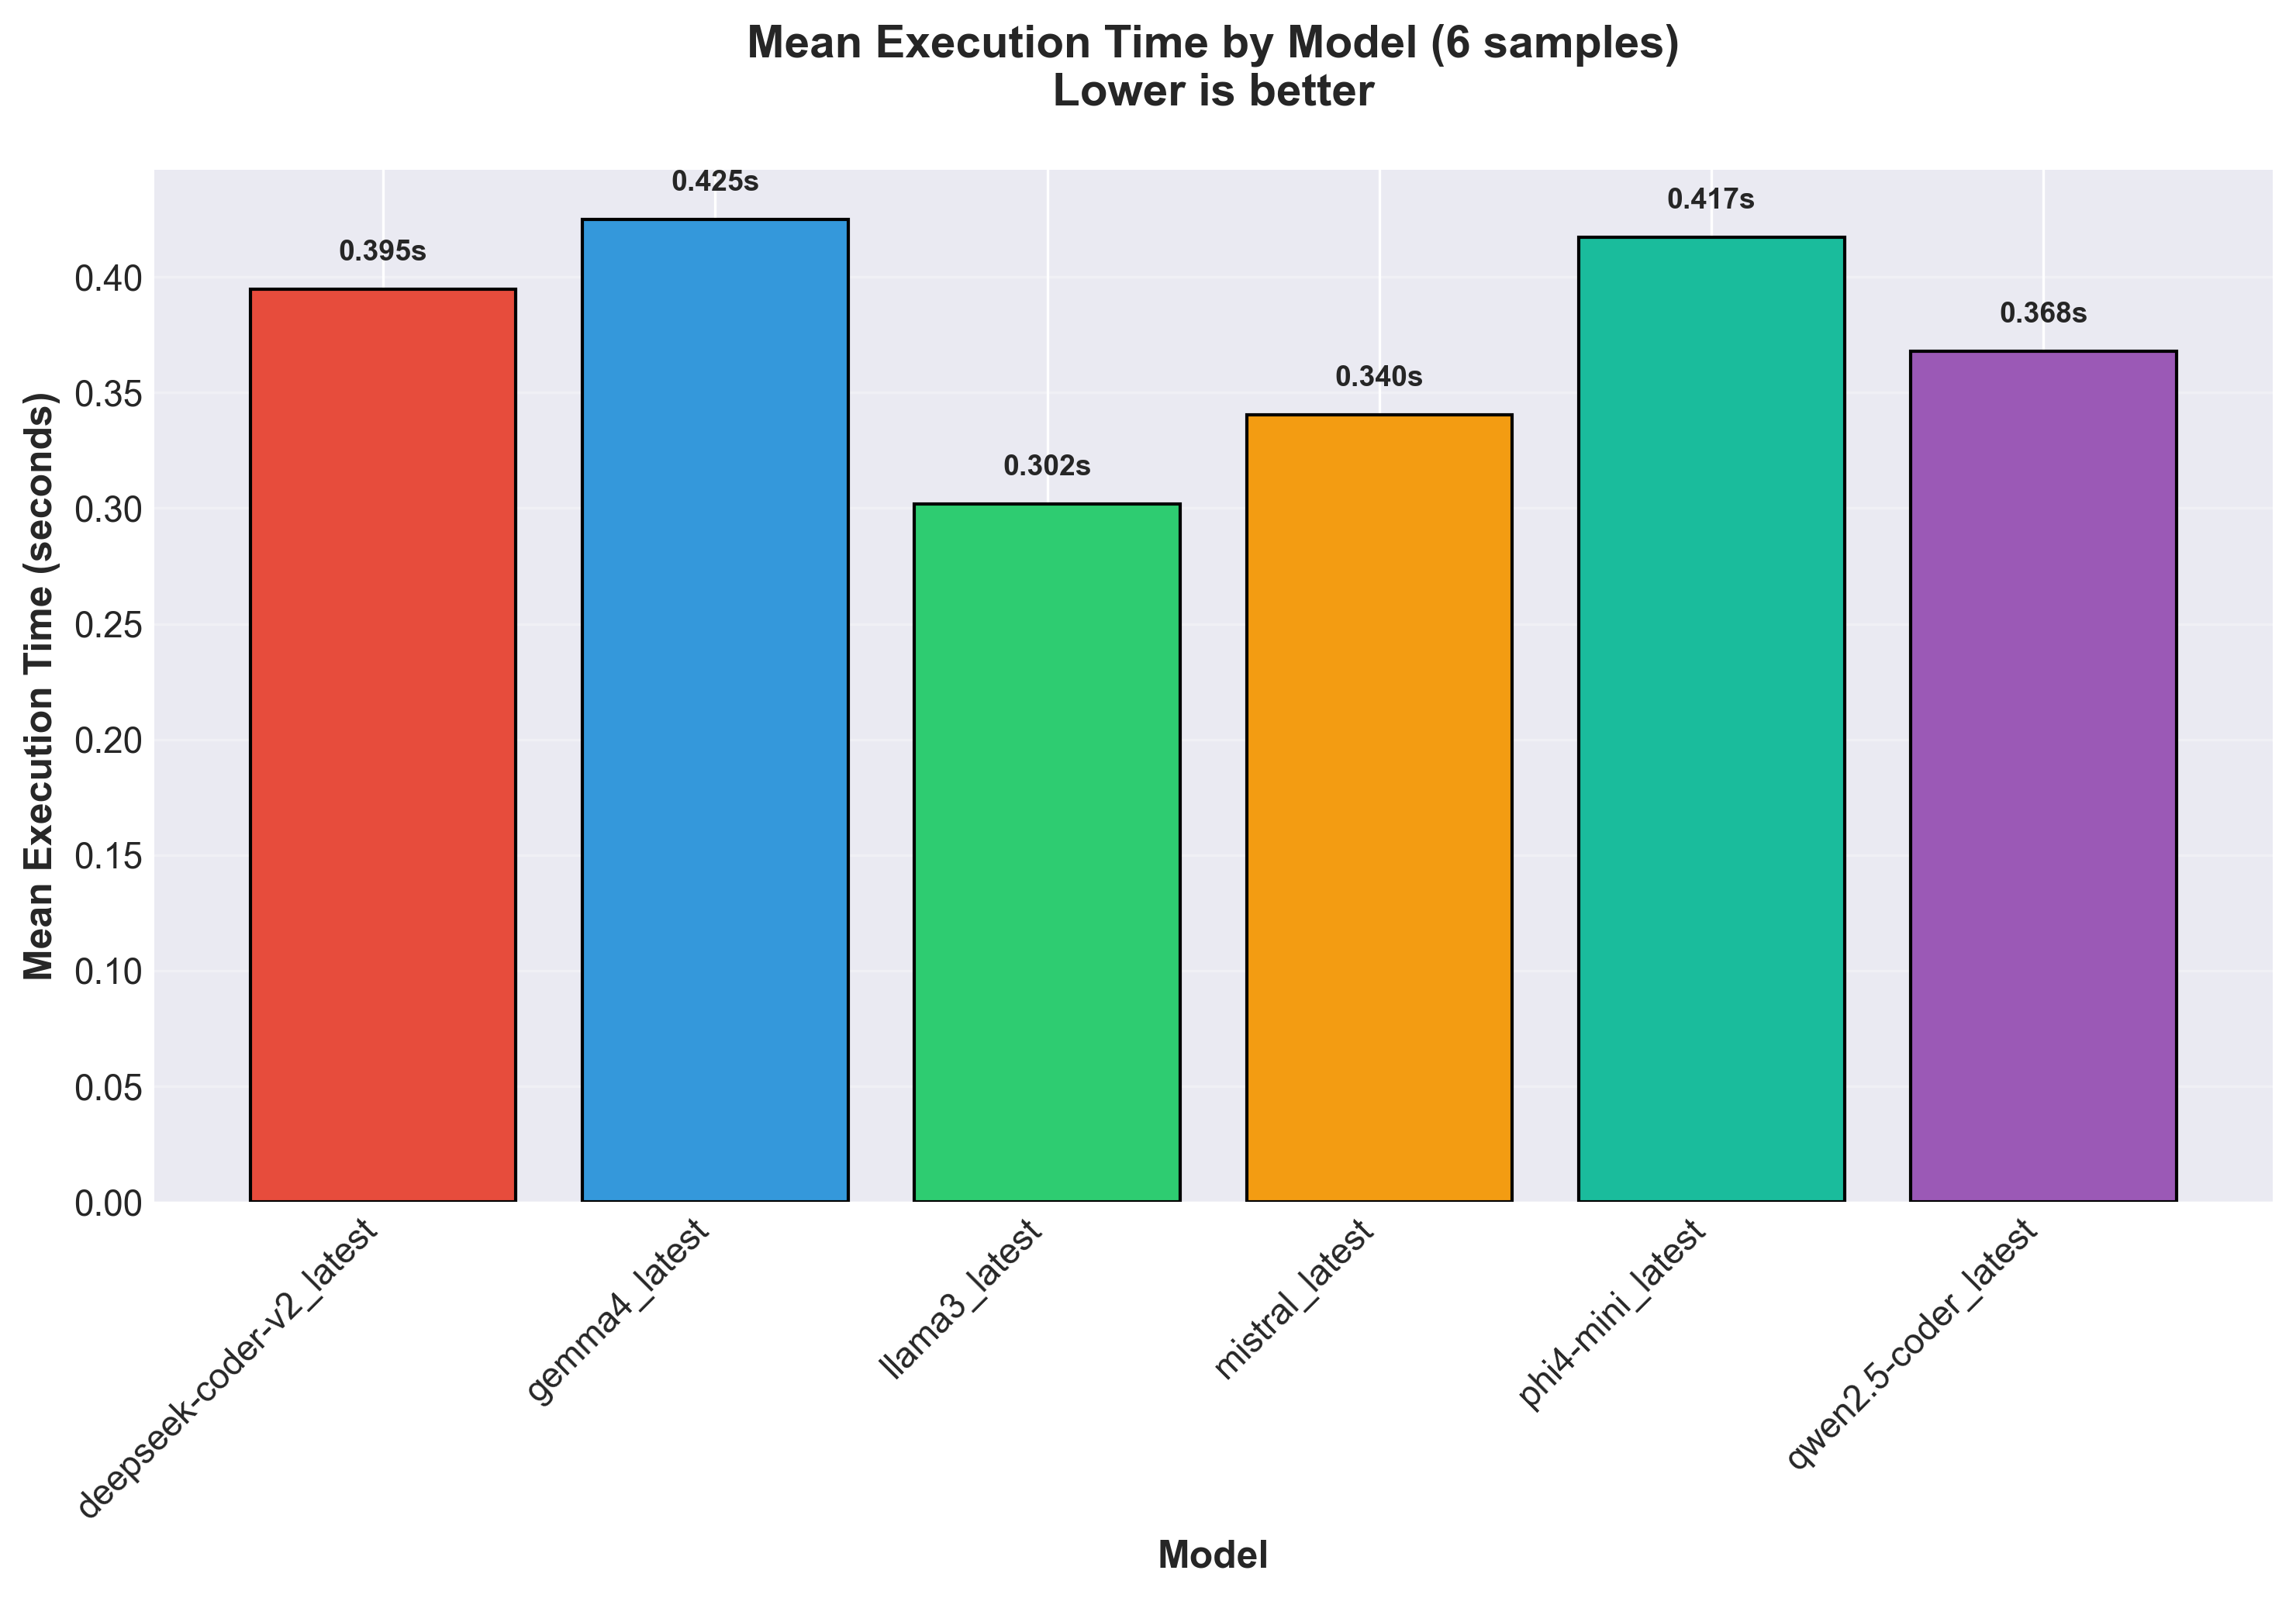
\includegraphics[width=0.9\linewidth]{images/06_execution_times.png}
    \caption{Uitvoeringstijden (seconden) per model. De figuur geeft inzicht in de runtime efficiëntie van de gegenereerde code.}
    \label{fig:execution_times}
\end{figure}

\begin{figure}[htbp]
    \centering
    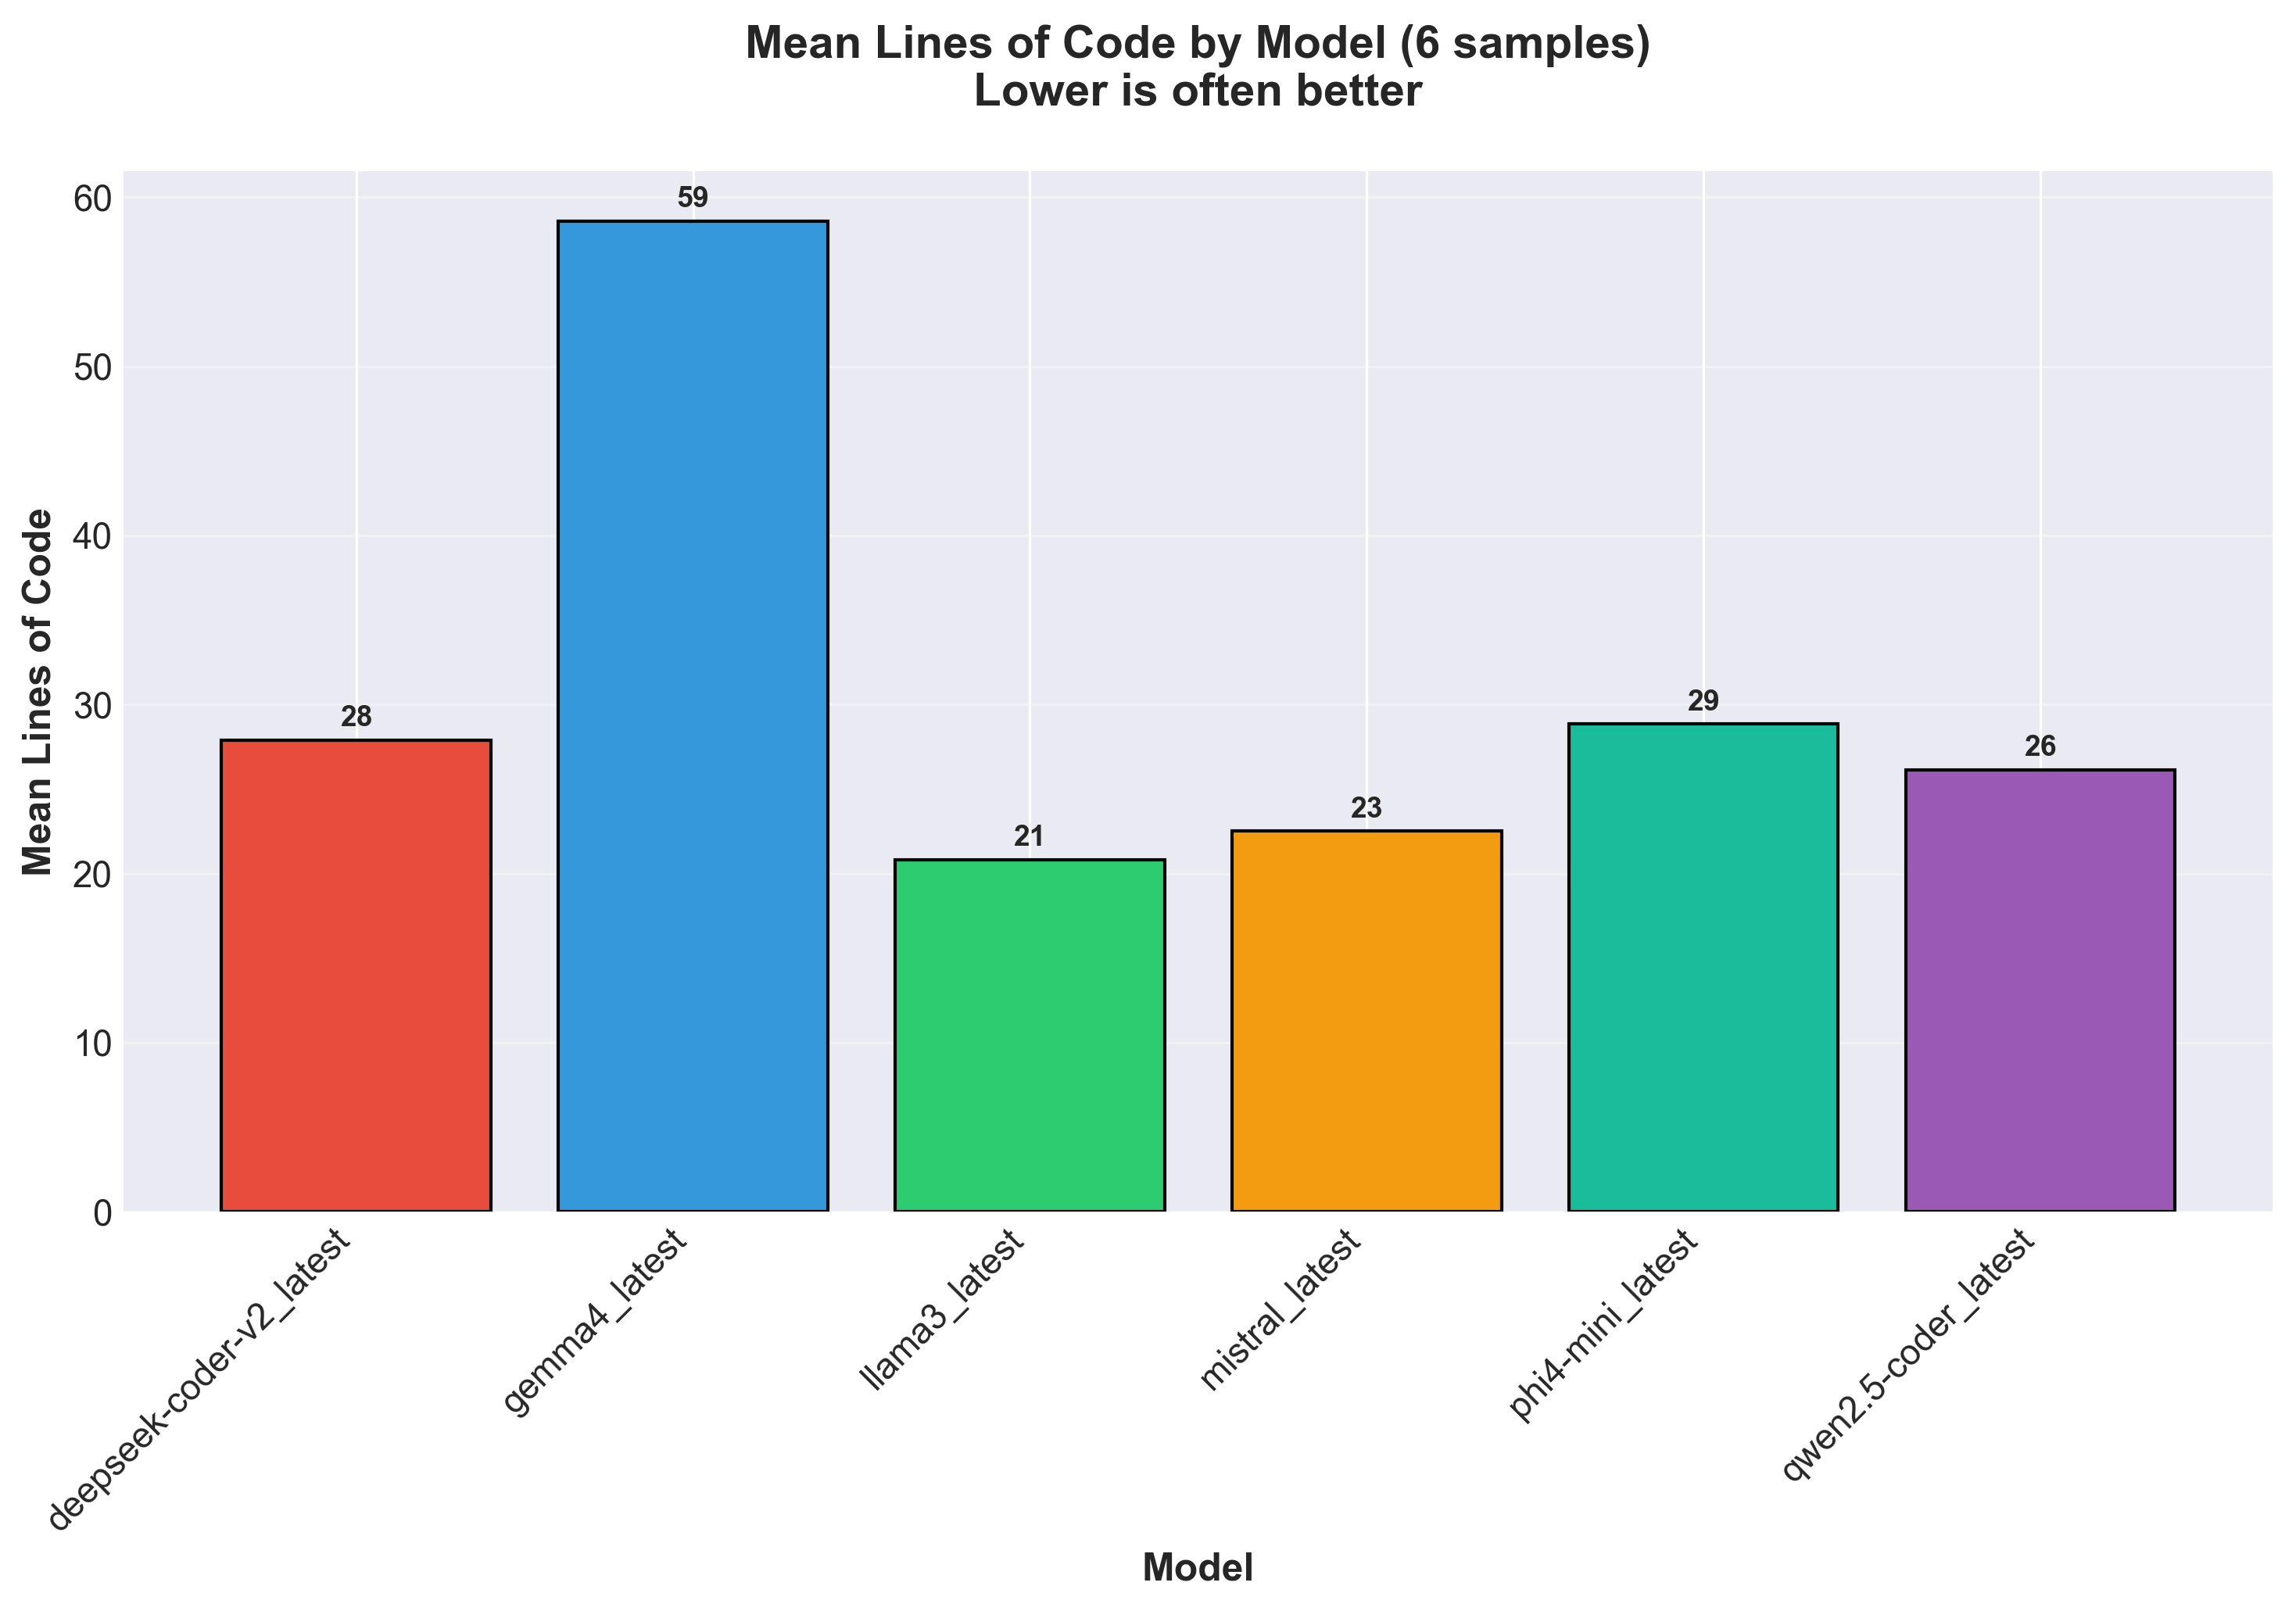
\includegraphics[width=0.9\linewidth]{images/07_lines_of_code.png}
    \caption{Plot van de code omvang (aantal regels) per model. De figuur toont het gemiddelde van het aantal regels per model.}
    \label{fig:lines_of_code}
\end{figure}

\begin{figure}[htbp]
    \centering
    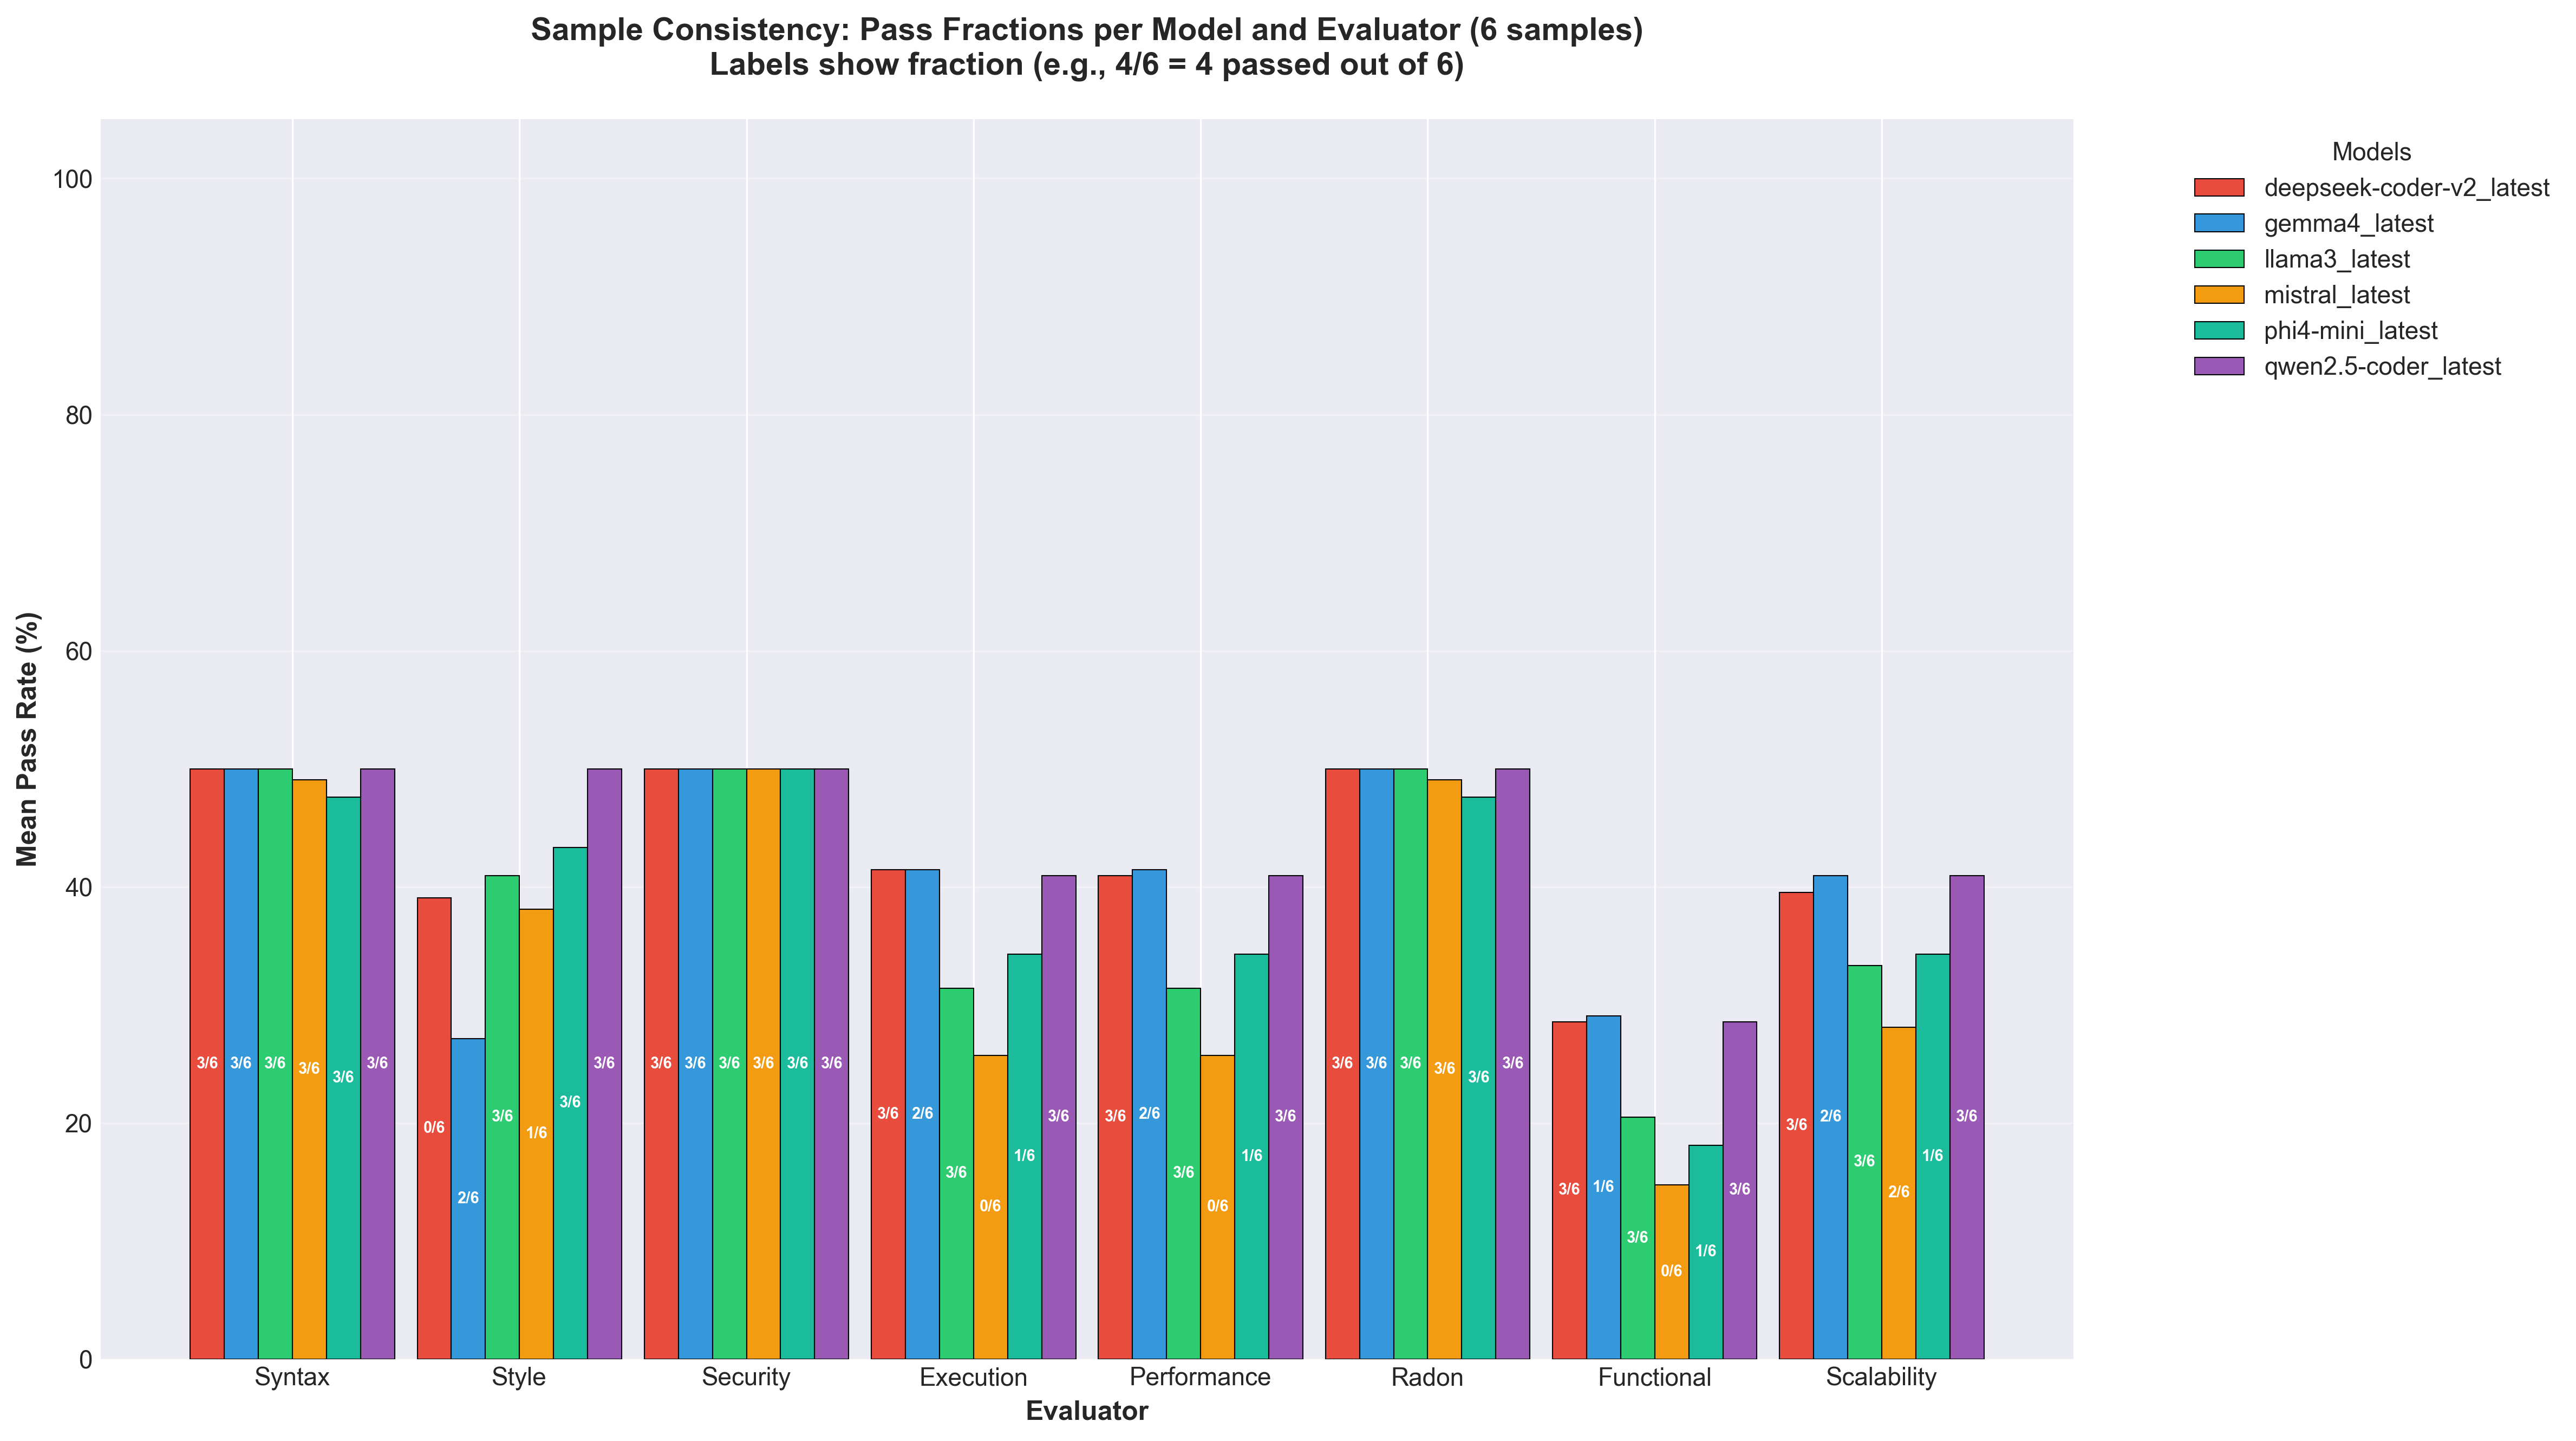
\includegraphics[width=0.9\linewidth]{images/08_sample_consistency.png}
    \caption{Consistentie van de drie gegenereerde samples per model en per evaluator. Een lagere waarde wijst op een betrouwbaardere codegeneratie.}
    \label{fig:08_sample_consistency}
\end{figure}

\begin{figure}[htbp]
    \centering
    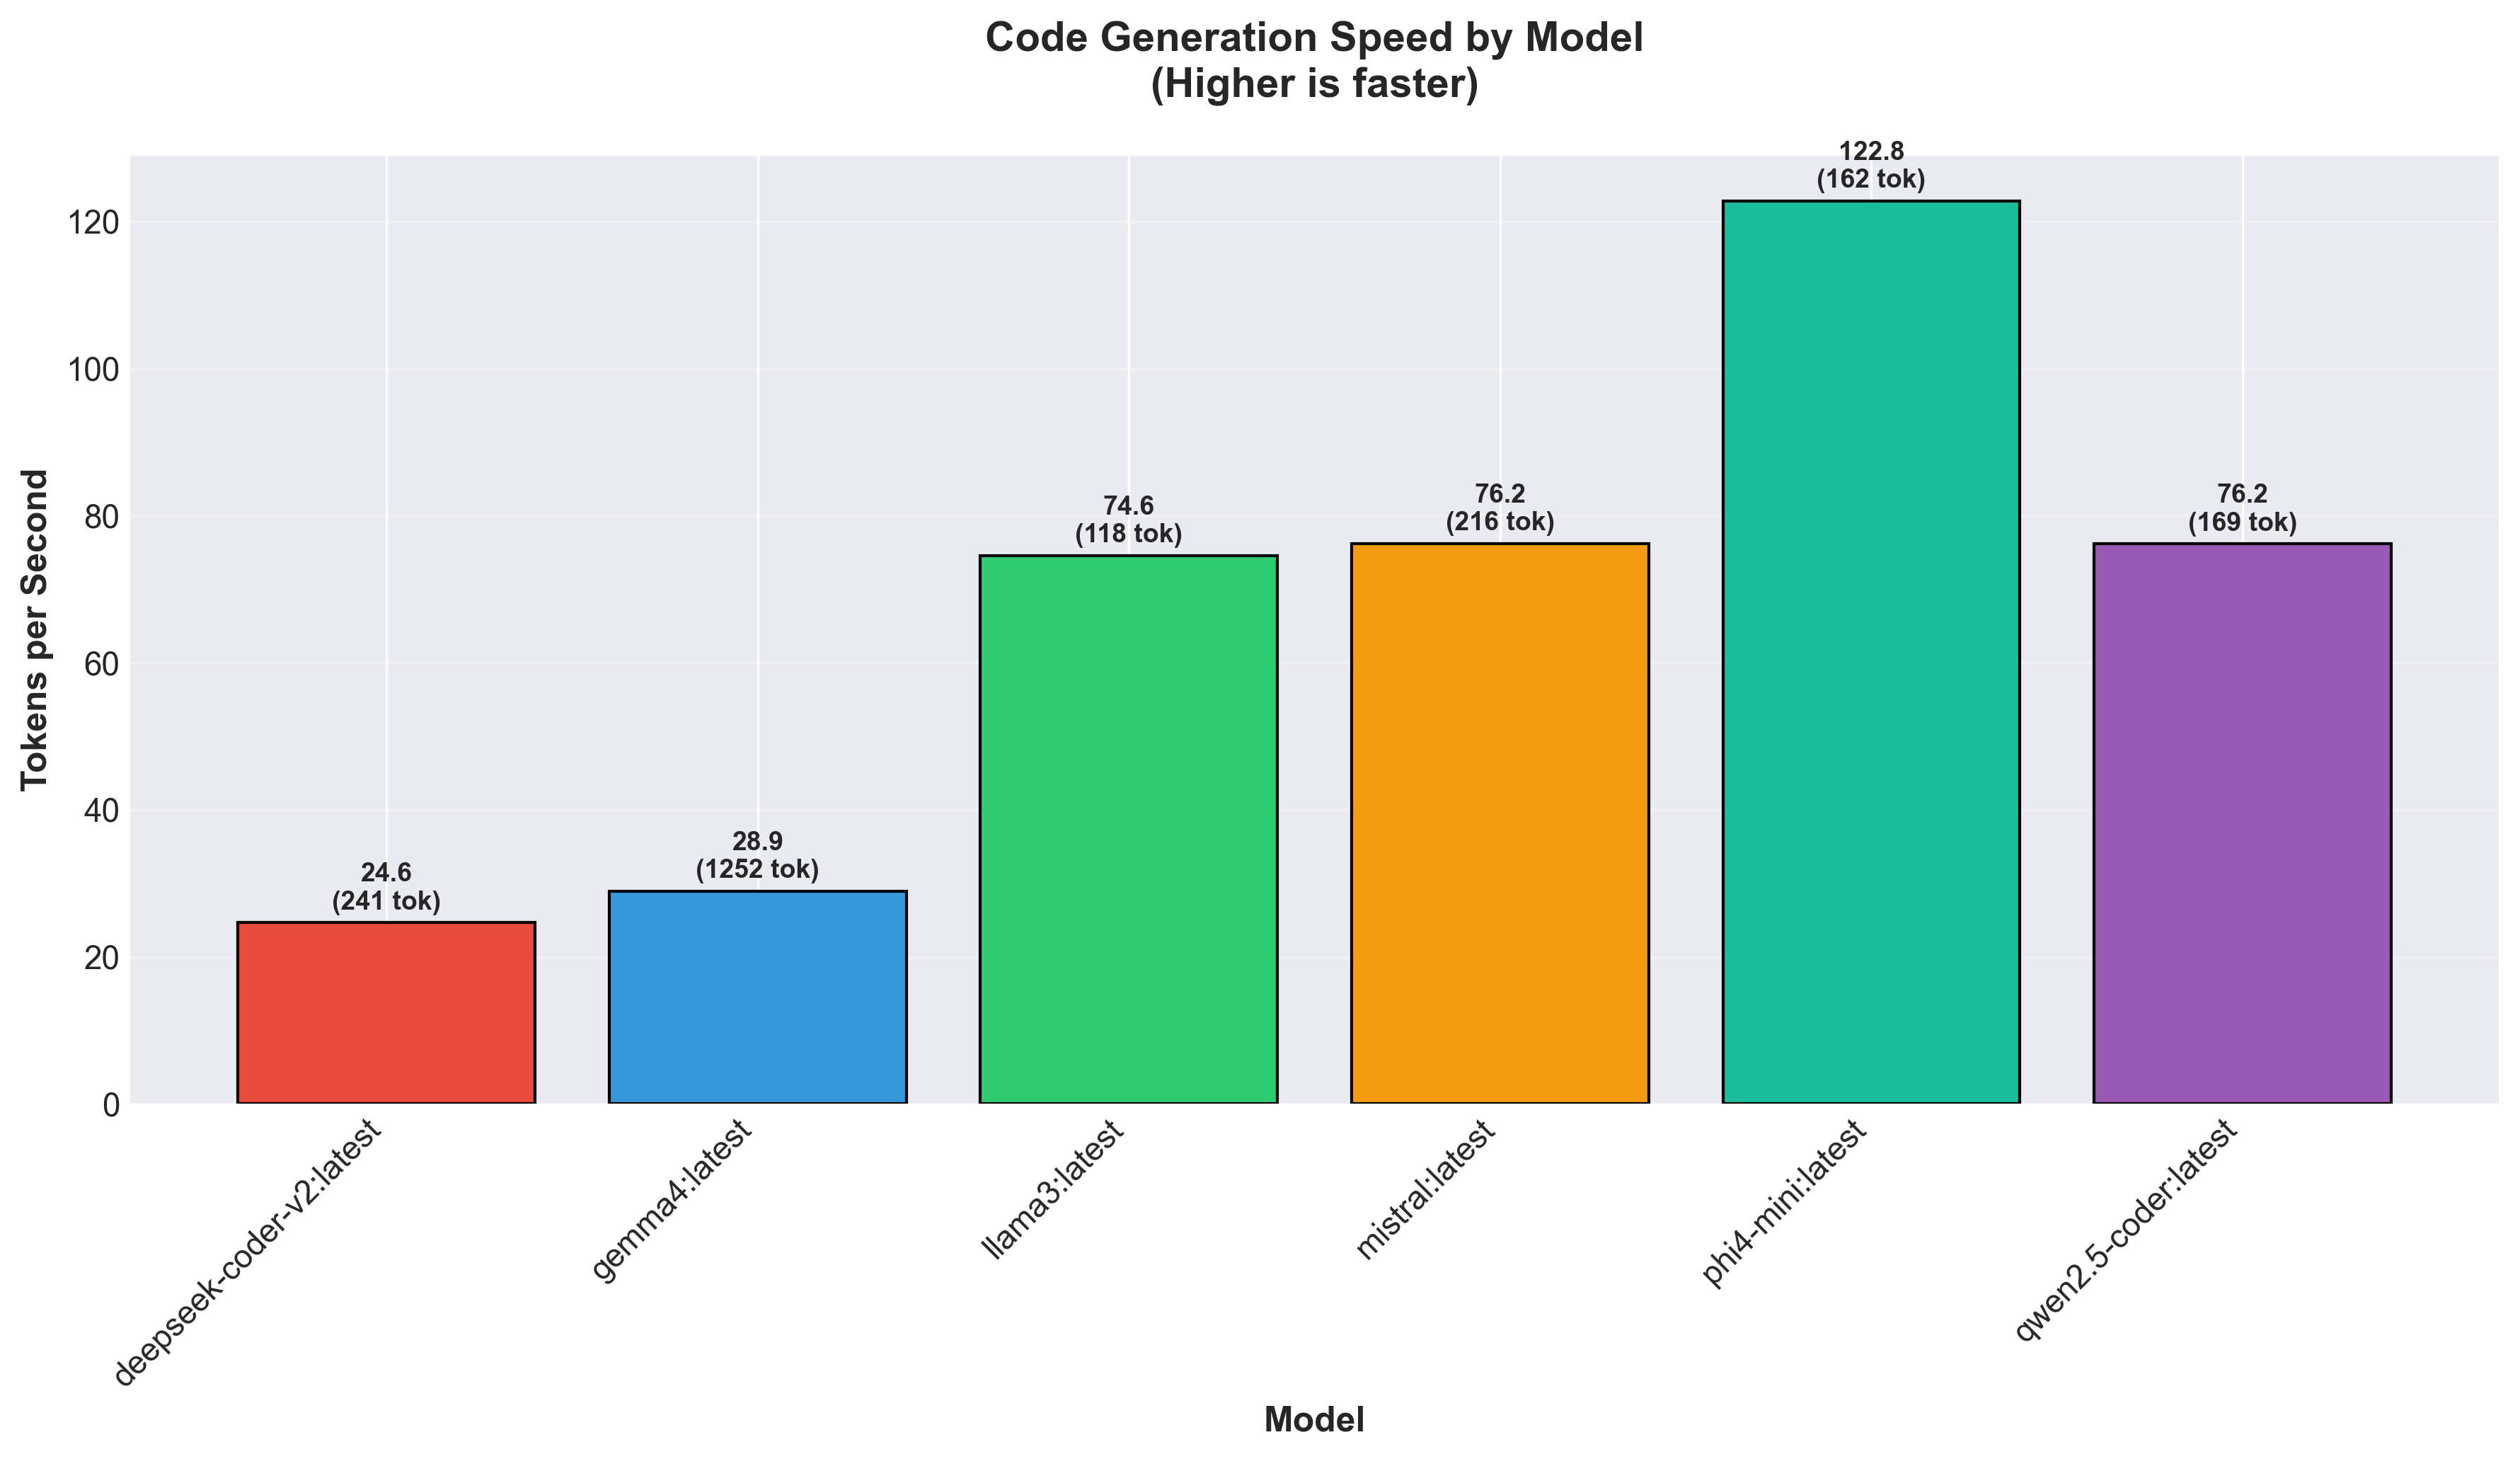
\includegraphics[width=0.9\linewidth]{images/09_generation_speed.png}
    \caption{Generatiesnelheid in tokens per seconde voor elk model. De figuur toont de verschillen in verwerkingssnelheid tussen de modellen.}
    \label{fig:09_generation_speed}
\end{figure}